%!TEX root = ../SciVis.tex
\subsection{Skeleton compilation}

use the standard version
recompiled the lib for x64 os x 
changing to framework 
different headerfiles

\subsection{Color mapping}
Color mapping is one of the most straight-forwards ways to visualize scalar values. This visualization technique maps each value to a specific color by using a scalar-to-color function (cf. Figure~\ref{fig:rainbowColormap}). 

We implemented this function as a lookup-table because we think that is is easier to define custom colormaps than compared to a transfer function. A disadvantage is that the lookup-table probably is more complex because it requires additional methods to manage the table.

We implemented the lookup-table as an array of 256 RGB color values. RGB has the advantage over HSV that it is additive, which makes linear interpolation easier. A colormap is defined by specifying a color at various points in the lookup table. These color points are stored in a map. The actual lookup-table will be generated by taking the color-points from the map and calculate the color by interpolating two adjacent color points. For instance blue at index 0, yellow at index 127 and green at index 255 will produce a colormap similar to the one shown in Figure~\ref{fig:colormaps}(d). 

\todo{the color points are stored in a map which is used to calculate the lookup table}

\begin{figure}[htbp]
    \centering
    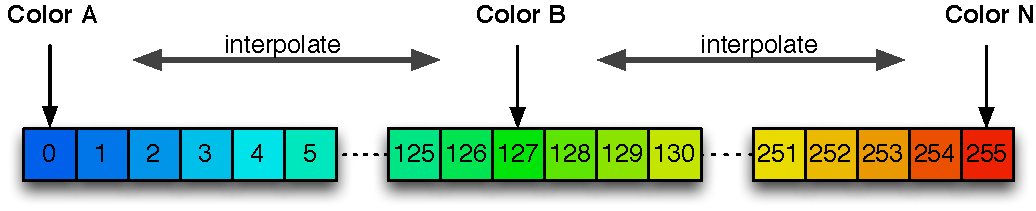
\includegraphics[width=.8\textwidth]{figures/colormaps/lookuptable.pdf}
    \caption{Conceptual model of the lookup-table. Missing colors are calculated by interpolating the defined color-points.}
    \label{fig:lookupTable}
\end{figure}

In the current implementation the colormaps are defined programmatically but it would be possible to easily create a user interface that lets the user define his own colormaps during runtime via drag and drop. The following colormaps have been predefined as illustrated in Figure~\ref{fig:colormaps}:
\begin{enumerate}[(a)]
    \item \textbf{Luminance (grayscale)} A simple universal colormap that adheres the linearity constraint. 
    \item \textbf{Rainbow} A colorful colormap that draws attention to high values as they are displayed in red. However, this colormap is often considered confusing due to unclear perceptual ordering of values and obscurity of data \footnote{Rainbow Color Map (Still) Considered Harmful, David Borland and Russell M., IEEE Computer Graphics and Applications} 
    \item \textbf{Heat} This type of colormap has a natural association with flames. Very high ``hot'' values are bright while lower values range from black to dark red.  
    \item \textbf{Blue-Yellow-Green} A colormap that separates the range of values into low, middle and high values. 
    \item \textbf{Black Gradient} A colormap that produces a gradient from any color to black.
    \item \textbf{White Gradient} A colormap that produces a gradient from any color to white.  
    \item \textbf{Zebra} A colormap that shows rapid value variations. This colormap makes it difficult to map certain regions to concrete values as low values cannot be distinguished from high values. 
\end{enumerate}   

\begin{figure}[htbp]
    \centering
    \begin{tabular}{ccccccc}
    
\includegraphics[height=1.75in]{figures/colormaps/grayscale.png}&
      
\includegraphics[height=1.75in]{figures/colormaps/rainbow.png}&
      
\includegraphics[height=1.75in]{figures/colormaps/heatmap.png}&         
     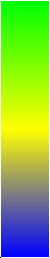
\includegraphics[height=1.75in]{figures/colormaps/blueYellowGreen.png}&
      
\includegraphics[height=1.75in]{figures/colormaps/blackGradient.png}&
      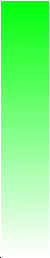
\includegraphics[height=1.75in]{figures/colormaps/whiteGradient.png}&
      
\includegraphics[height=1.75in]{figures/colormaps/zebra.png}\\
    (a)&(b)&(c)&(d)&(e)&(f)&(g)\\
    \end{tabular}
    \caption{Predefined colormaps: (a) Luminance, (b) Rainbow, (c) Heatmap, (d)  Blue-Green-Yellow, (e) Black Gradient (f) White Gradient (g) Zebra}
    \label{fig:colormaps}
\end{figure}


Furthermore the user has the possibility to change hue and saturation of the  colormap during runtime. In order to apply hue ($h$) and saturation ($s$), the colors are translated into the HSV color system. Due to the circular nature of the hue, $h$ shifts the color($c$) along the hue color wheel. Instead saturation is applied by multiplication, which implies that the saturation can only be decreased for any color.

\begin{eqnarray*}
c_{hue} &=&  (c_{hue} + h)~\%~1\\
c_{sat} &=& c_{sat} * s
\end{eqnarray*}
A less saturated and hue shifted version of the rainbow colormap is illustrated in Figure~\ref{fig:saturationAndHueColormap}.

\begin{figure}[htbp]
\centering
\begin{minipage}[t]{0.48\textwidth}
        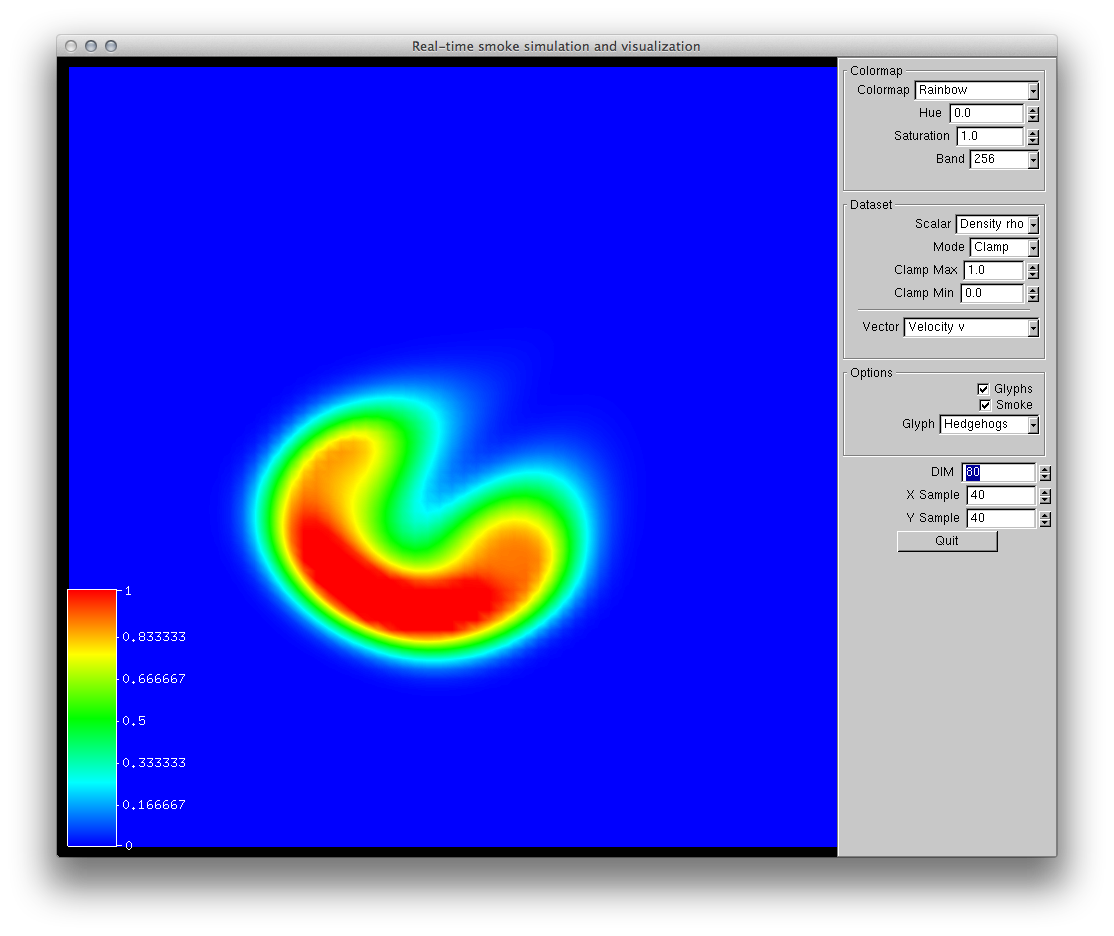
\includegraphics[height=3in]{figures/colormaps/rainbowSmoke.png}
\caption{Fluid density visualized with a rainbow colormap.}
\label{fig:rainbowColormap}
\end{minipage}\hspace{.04\textwidth}%
\begin{minipage}[t]{0.48\textwidth}
        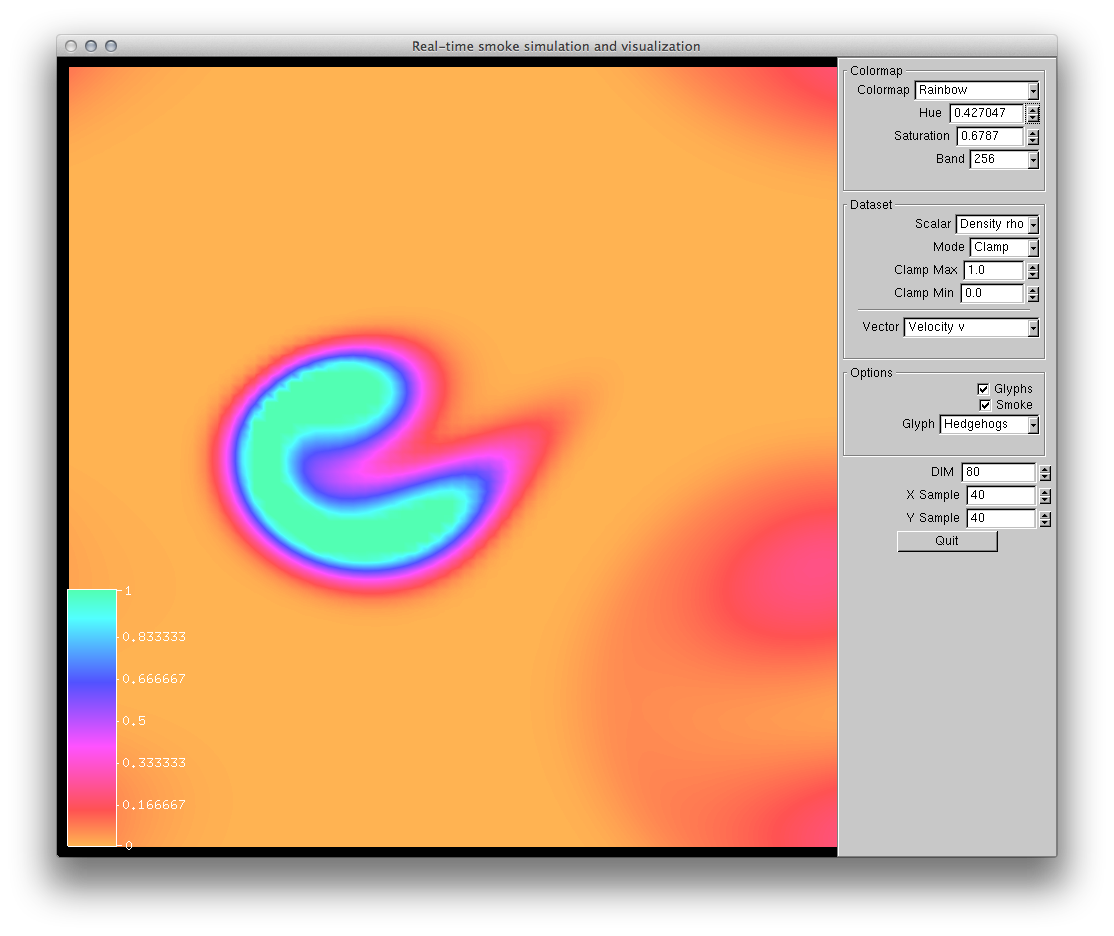
\includegraphics[height=3in]{figures/colormaps/hueAndSaturation.png}
    \caption{Fluid density with a less-saturated and hue-shifted rainbow colormap.}
    \label{fig:saturationAndHueColormap}
\end{minipage}
\end{figure}


One is the fundamental problems is to map the values to a particular color, especially if the range of values is not known in advance or the dataset contains a few but extreme peaks or valley. Two different mapping modes have been implemented, which are clamping and scaling. Clamping allows the user to specify the minimum and maximum value, all values larger or smaller are clamped to the maximum respectively to the minimum value. 
In contrast, scaling uses the complete range of values in the dataset of the current timestep. This means that we have to calculate the current minimum and maximum value for every timestep before we map the values to a color.

The minimum and maximum value is necessary in order to translate the value range to the color range. This is done by scaling the value range up or down to the range of 0 to 255 by using the following code snippet. The resulting float value is rounded to its nearest integer value, which determines the index within the color table. 

\begin{lstlisting}][language=C]
float scale(float v, float f_min, float f_max, float min, float max) {
    return ((v - f_min)*(max - min) / (f_max - f_min) + min);
}
\end{lstlisting}

Figure~\ref{fig:forceScaled} depicts the visualization of the force magnitude by using a rainbow colormap and the scaling mode. The displayed colors extend over the complete range of available colors, although the values are very small and the range of values is quite narrow. During runtime it can be observed that the legend is constantly updated as the values become increasingly smaller unless new force is added. 

\begin{figure}[htbp]
\centering
\begin{minipage}[t]{0.48\textwidth}
        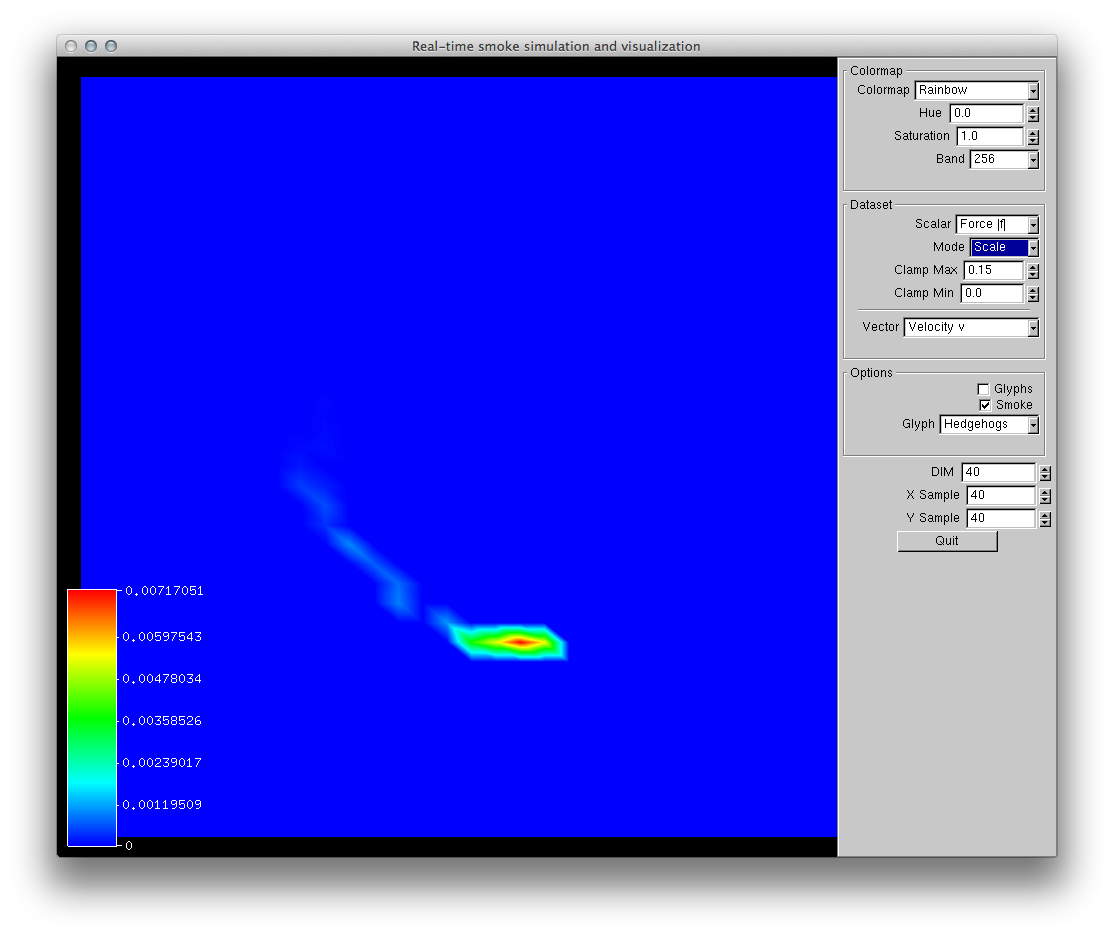
\includegraphics[height=3in]{figures/colormaps/forceScaled.png}
\caption{Scaling the colormap to the min and max of force always shows the maximum and minimum values at the current timestep although the values are quite small.}
\label{fig:forceScaled}
\end{minipage}\hspace{.04\textwidth}%
\begin{minipage}[t]{0.48\textwidth}
        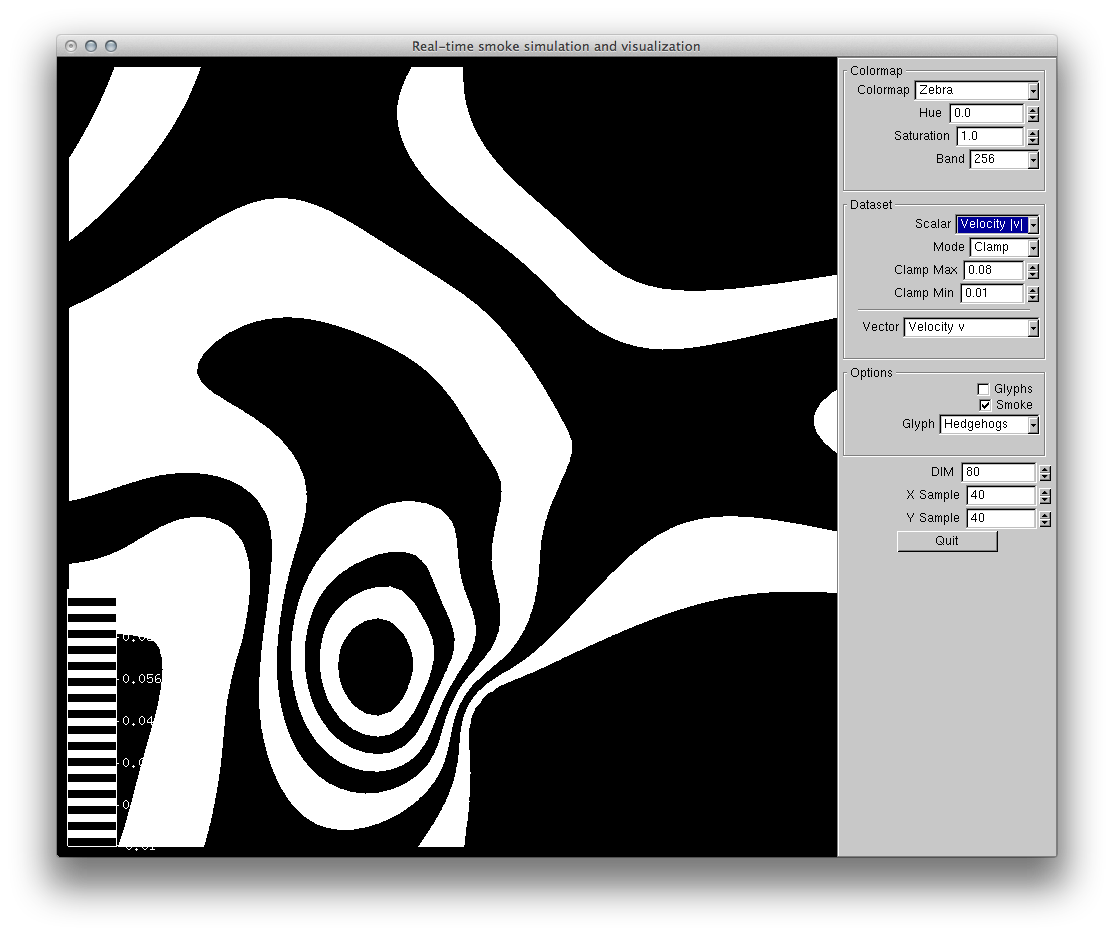
\includegraphics[height=3in]{figures/colormaps/velocityZebra.png}
    \caption{Velocity visualized with a zebra colormap that highlights areas with high variation.}
    \label{fig:velocityZebra}
\end{minipage}
\end{figure}

In order to increase the accuracy we have implemented texture-based color mapping rather than vertex-based color mapping. The advantage is that not the color is interpolated between sample points but instead the index of the color. This produces better results as the mapped color is always part of the colormap. This is not automatically the case for vertex-based color mapping and thus requires a more careful design of the colormap itself. In order to use texture-based mapping we need to generate a texture whenever the colormap is changed (e.g. different colormap, hue, saturation, number of colors). 
The colormap is generated based on the lookup-table. 

Another  parameter that the user can influence is the  number of colors, the less colors are specified in a colormap the more banding artifacts will be visible (cf.~Figure~\ref{fig:banding}, \ref{fig:heatmap}). 
We implemented banding by reducing the number of different colors in the lookup-table. The size of the lookup table itself always stays the same, which is 256 cells. This has the advantage that we do not need adapt the code for scaling or generating textures. 
As an example, we want to reduce the number of colors to 32. In concrete, this means the every eighth color in the base lookup-table will be spread over the following eight cells. The code is illustrated in Listing~\ref{lst:banding}


\begin{lstlisting}[language=C,label=lst:banding,caption={Reducing the number of colors in the lookup-table}]
int step = 256 / numberOfColors;
 for (size_t i = 0; i < 256; i++) {

     int c = step * (int) floor(i / step);
     if (i >= 128) {
         c = c + step - 1;
     }
     colors[i] = colors[c];
 }
 \end{lstlisting}

One of the most important aspects of visualization is the invert mapping of colors to data values in order to generate insight. A color legend allows to associate concrete colors with values by showing both the colormap itself and the corresponding numerical values as shown in Figure~\ref{fig:heatmap}.. However, the invert mapping is only possible with limited accuracy because it is not feasible to display all numerical values. The color legend is based on the lookup-table and the current minimum and maximum values of the dataset. Based on this information, the major and minor tick marks are calculated.

\begin{figure}[htbp]
\centering
\begin{minipage}[t]{0.48\textwidth}
        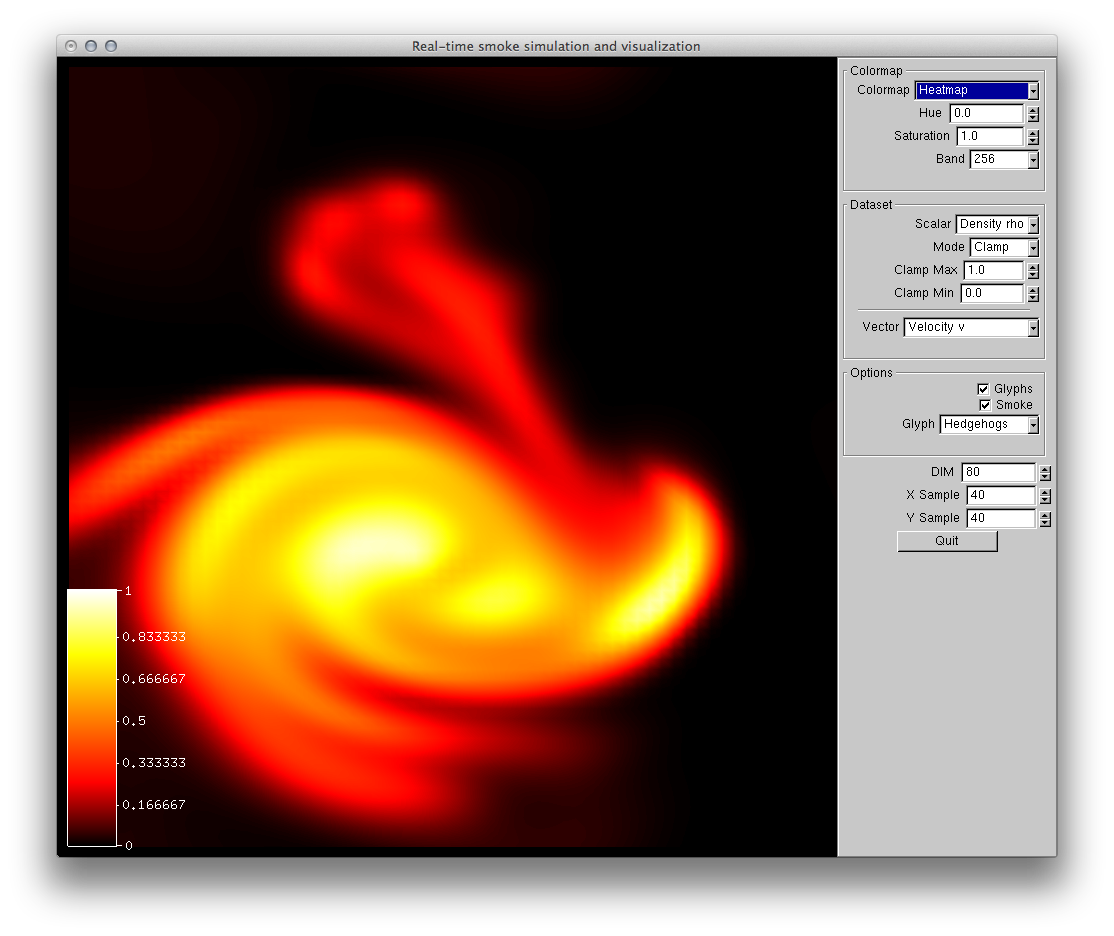
\includegraphics[height=3in]{figures/colormaps/heatmapSmoke.png}
\caption{Fluid density visualized with a heat colormap}
\label{fig:heatmap}
\end{minipage}\hspace{.04\textwidth}%
\begin{minipage}[t]{0.48\textwidth}
        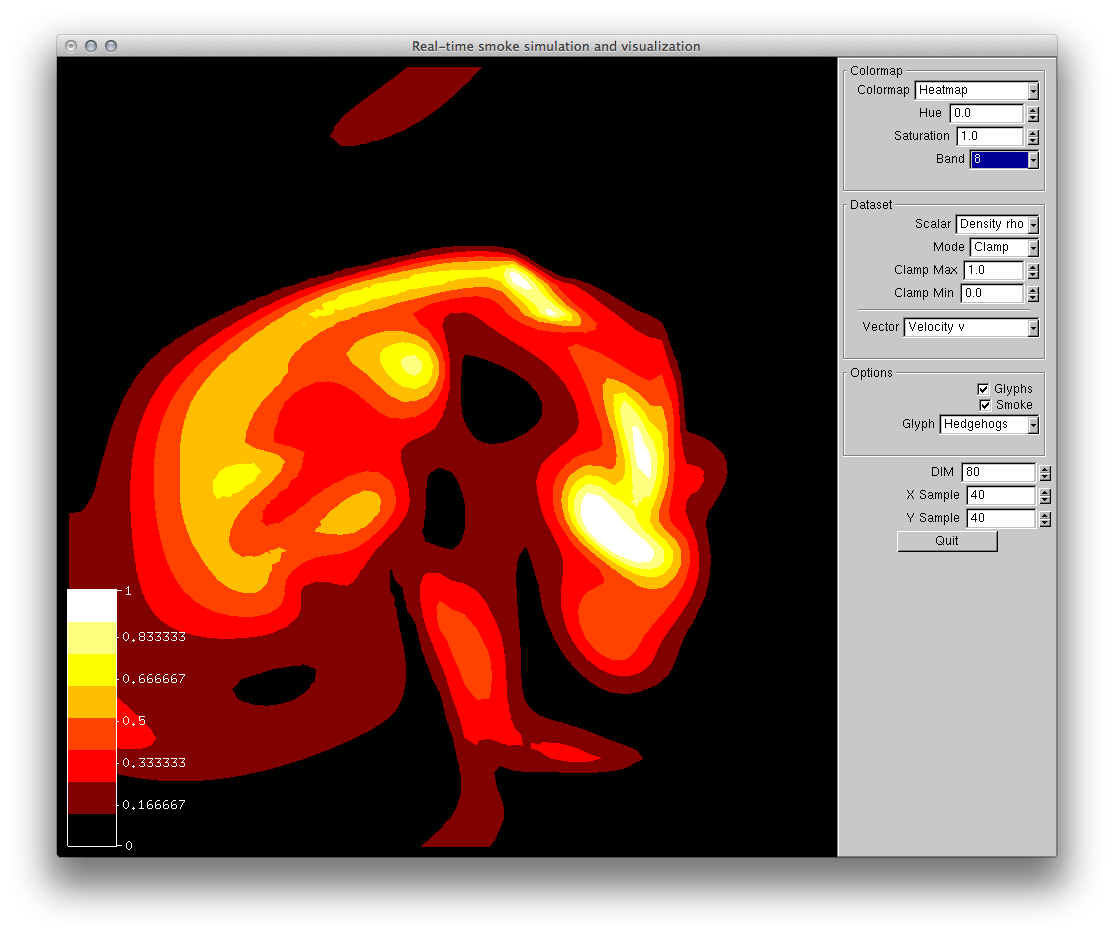
\includegraphics[height=3in]{figures/colormaps/heatmapSmokeBanded.png}
    \caption{Heat colormap with a reduced number of colors. The color banding effect is clearly visible.}
    \label{fig:banding}
\end{minipage}
\end{figure}

\clearpage

\subsection{Glyphs}

The vector glyph technique associates vector glyphs with sample points of a vector dataset. Glyphs are able of conveying, by their appearance, properties of the represented vector, such as direction, orientation, and magnitude. However, when using vector glyphs the task of image-to-data mapping is getting harder, especially when it is needed to interpolate between orientations and directions. The Smoke application contains two vector datasets ---velocity and force. Four different kind of glyphs are used ---hedgehogs, simple arrows, 3D cones, and 3D arrows.

In order to use the glyph visualisation technique, the user must select the option \emph{Glyphs} from the \emph{Options} panel. The user is able to select which kind of glyph will be used for the visualisation from the \emph{Glyph} listbox which can be found in the \emph{Dataset} panel. The user is also able to select which vector dataset to visualise regardless of the selected glyph icon. This is possible from the \emph{Vector} listbox which can be found in the \emph{Dataset} panel. For colouring the glyphs, the user can select one of the scalar datasets ---density, velocity magnitude, force magnitude, and velocity divergence.

The simplest glyph icon used is the hedgehogs. Figure~\ref{fig:hedgehogs} shows hedgehogs during the visualisation of the \emph{velocity} vector dataset. The \emph{density} scalar dataset is used for colouring the glyphs and the rainbow colormap was used. Hedgehogs are able to show the position, direction, and magnitude of a set of vectors. The grid is regularly sampled on a 60x60 dimension. This due to the reason that high resolution vector datasets are better visualised when subsampled. We could have sample the grid in 80x80 dimensions, but then we would have to decrease the glyph scaling factor, so we could avoid cluttering issues.

\begin{figure}[htbp]
\begin{center}
 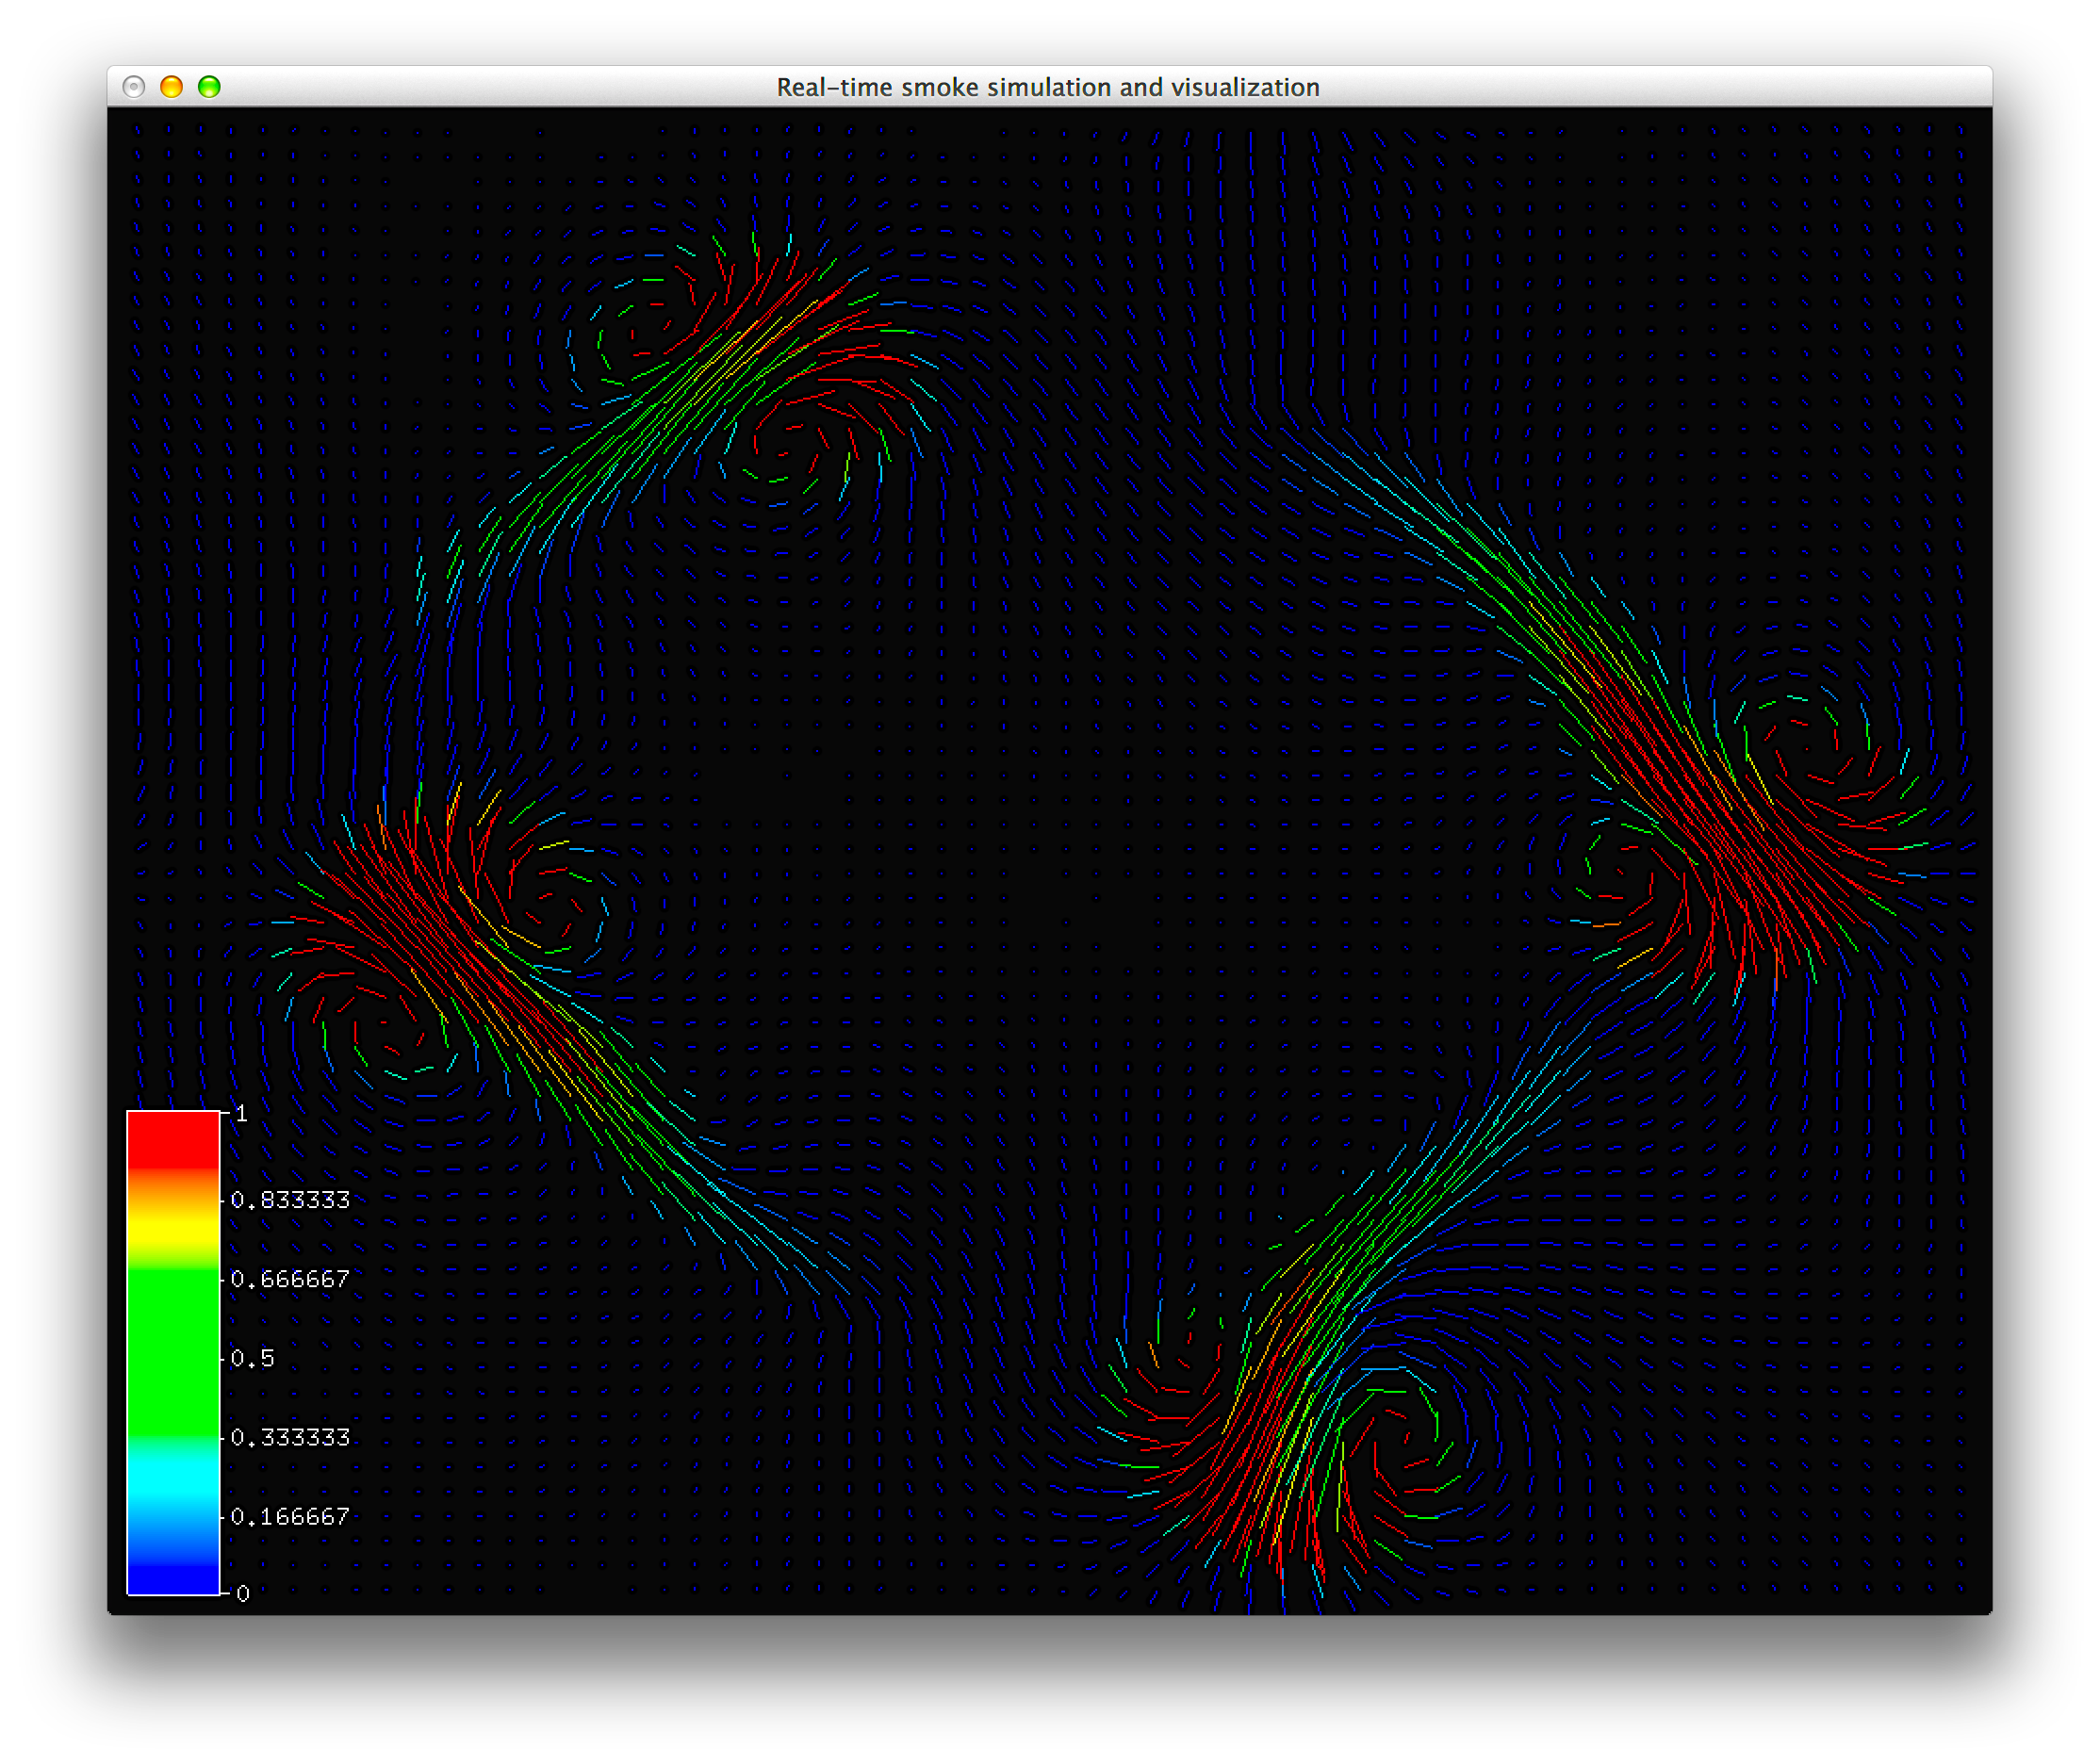
\includegraphics[height=3.5in]{figures/glyph/hedgehogsRainbow.png}
\caption{Hedgehog visualisation of smoke simulation using rainbow colouring. Regularly sampled on 60x60 and scaling factor 1000.}
\label{fig:hedgehogs}
\end{center}
\end{figure}

Scaling factor is an option that needs careful consideration when visualising glyphs. As can be seen from Figure~\ref{fig:hedgehogs} it is very easy to follow the direction of the vector dataset using a linear scaling factor of 1000. Although the hedgehogs are drawn on top of each other, where the magnitude of the vector field gets its highest values, the direction of the vector field is still clearly visible. However, as it is depicted in Figure~\ref{fig:hedgehogsSamplesScaling}(b), when increasing the number of samples and retaining the scaling factor at 1000 cluttering becomes an issue. In Figure~\ref{fig:hedgehogsSamplesScaling}(a), the visualisation shows the same dataset regularly sampled on 40x40 and with a scaling factor of 200. In this case cluttering effects have been eliminated, but we are not able anymore to use the glyph length as a visual cue for the vector field magnitude.

\begin{figure}[htbp]
\centering
\begin{minipage}[t]{0.48\textwidth}
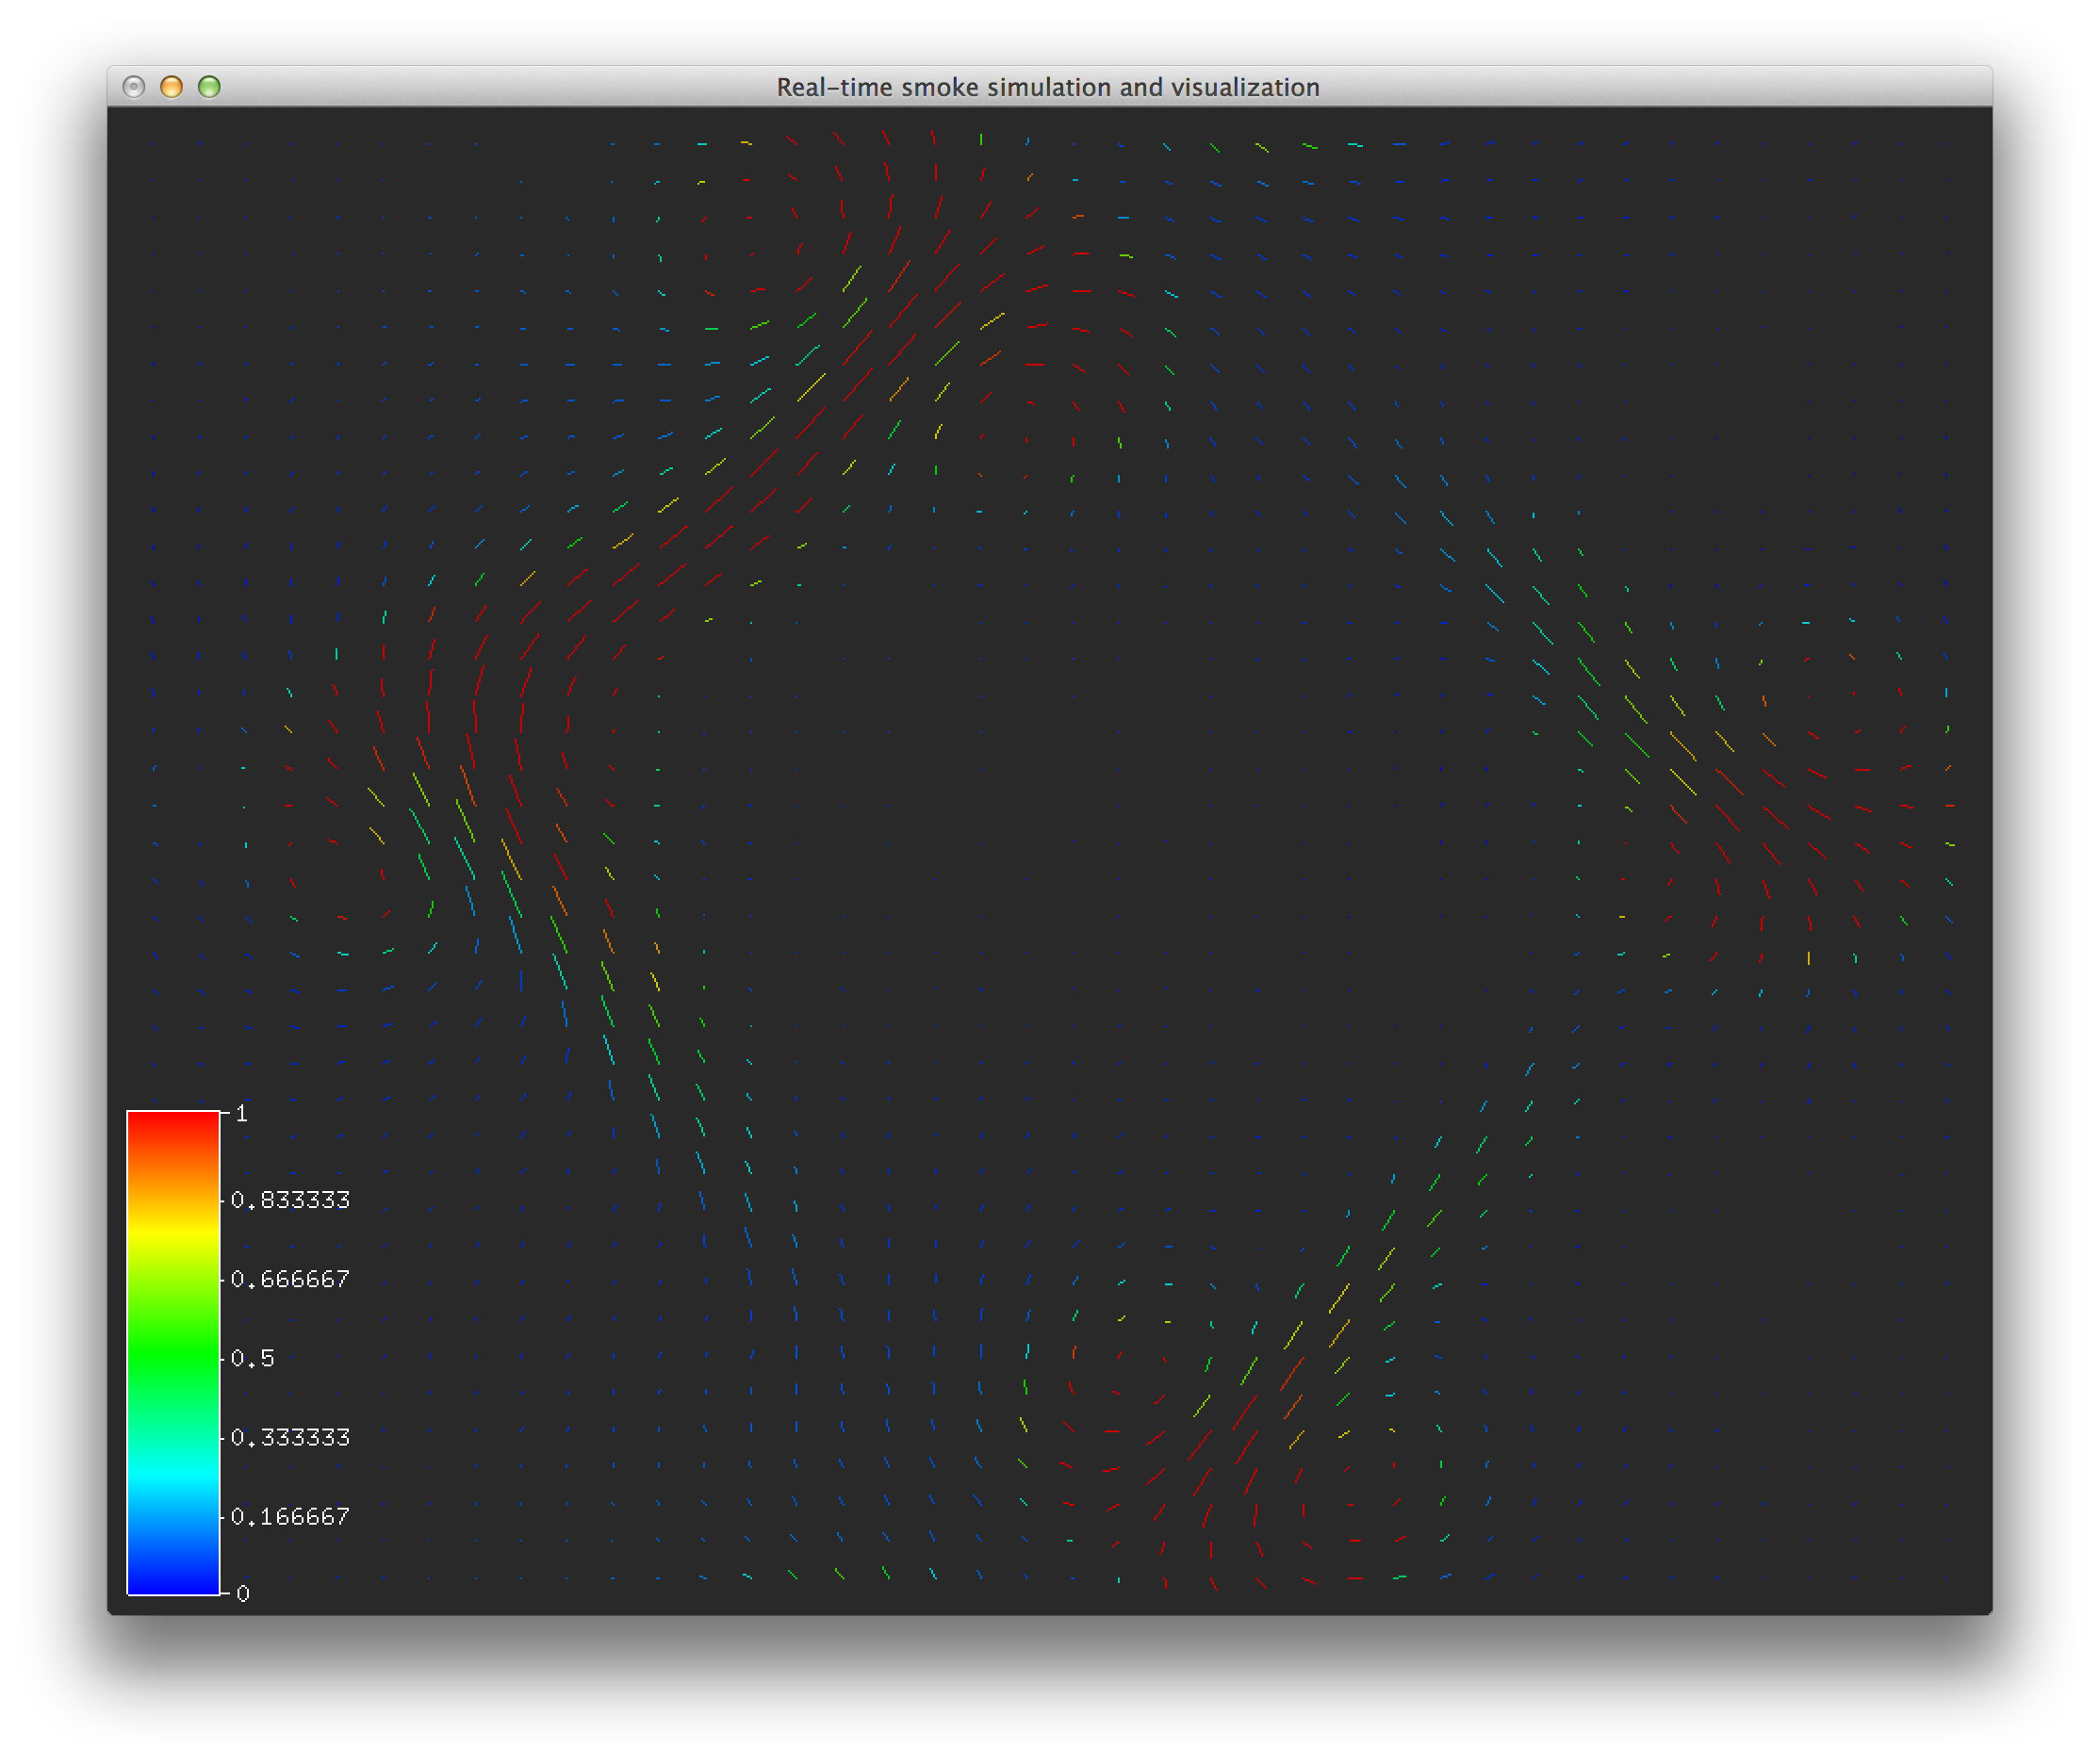
\includegraphics[height=2.7in]{figures/glyph/hedgehogsLSSSF.png}
\end{minipage}
\begin{minipage}[t]{0.48\textwidth}
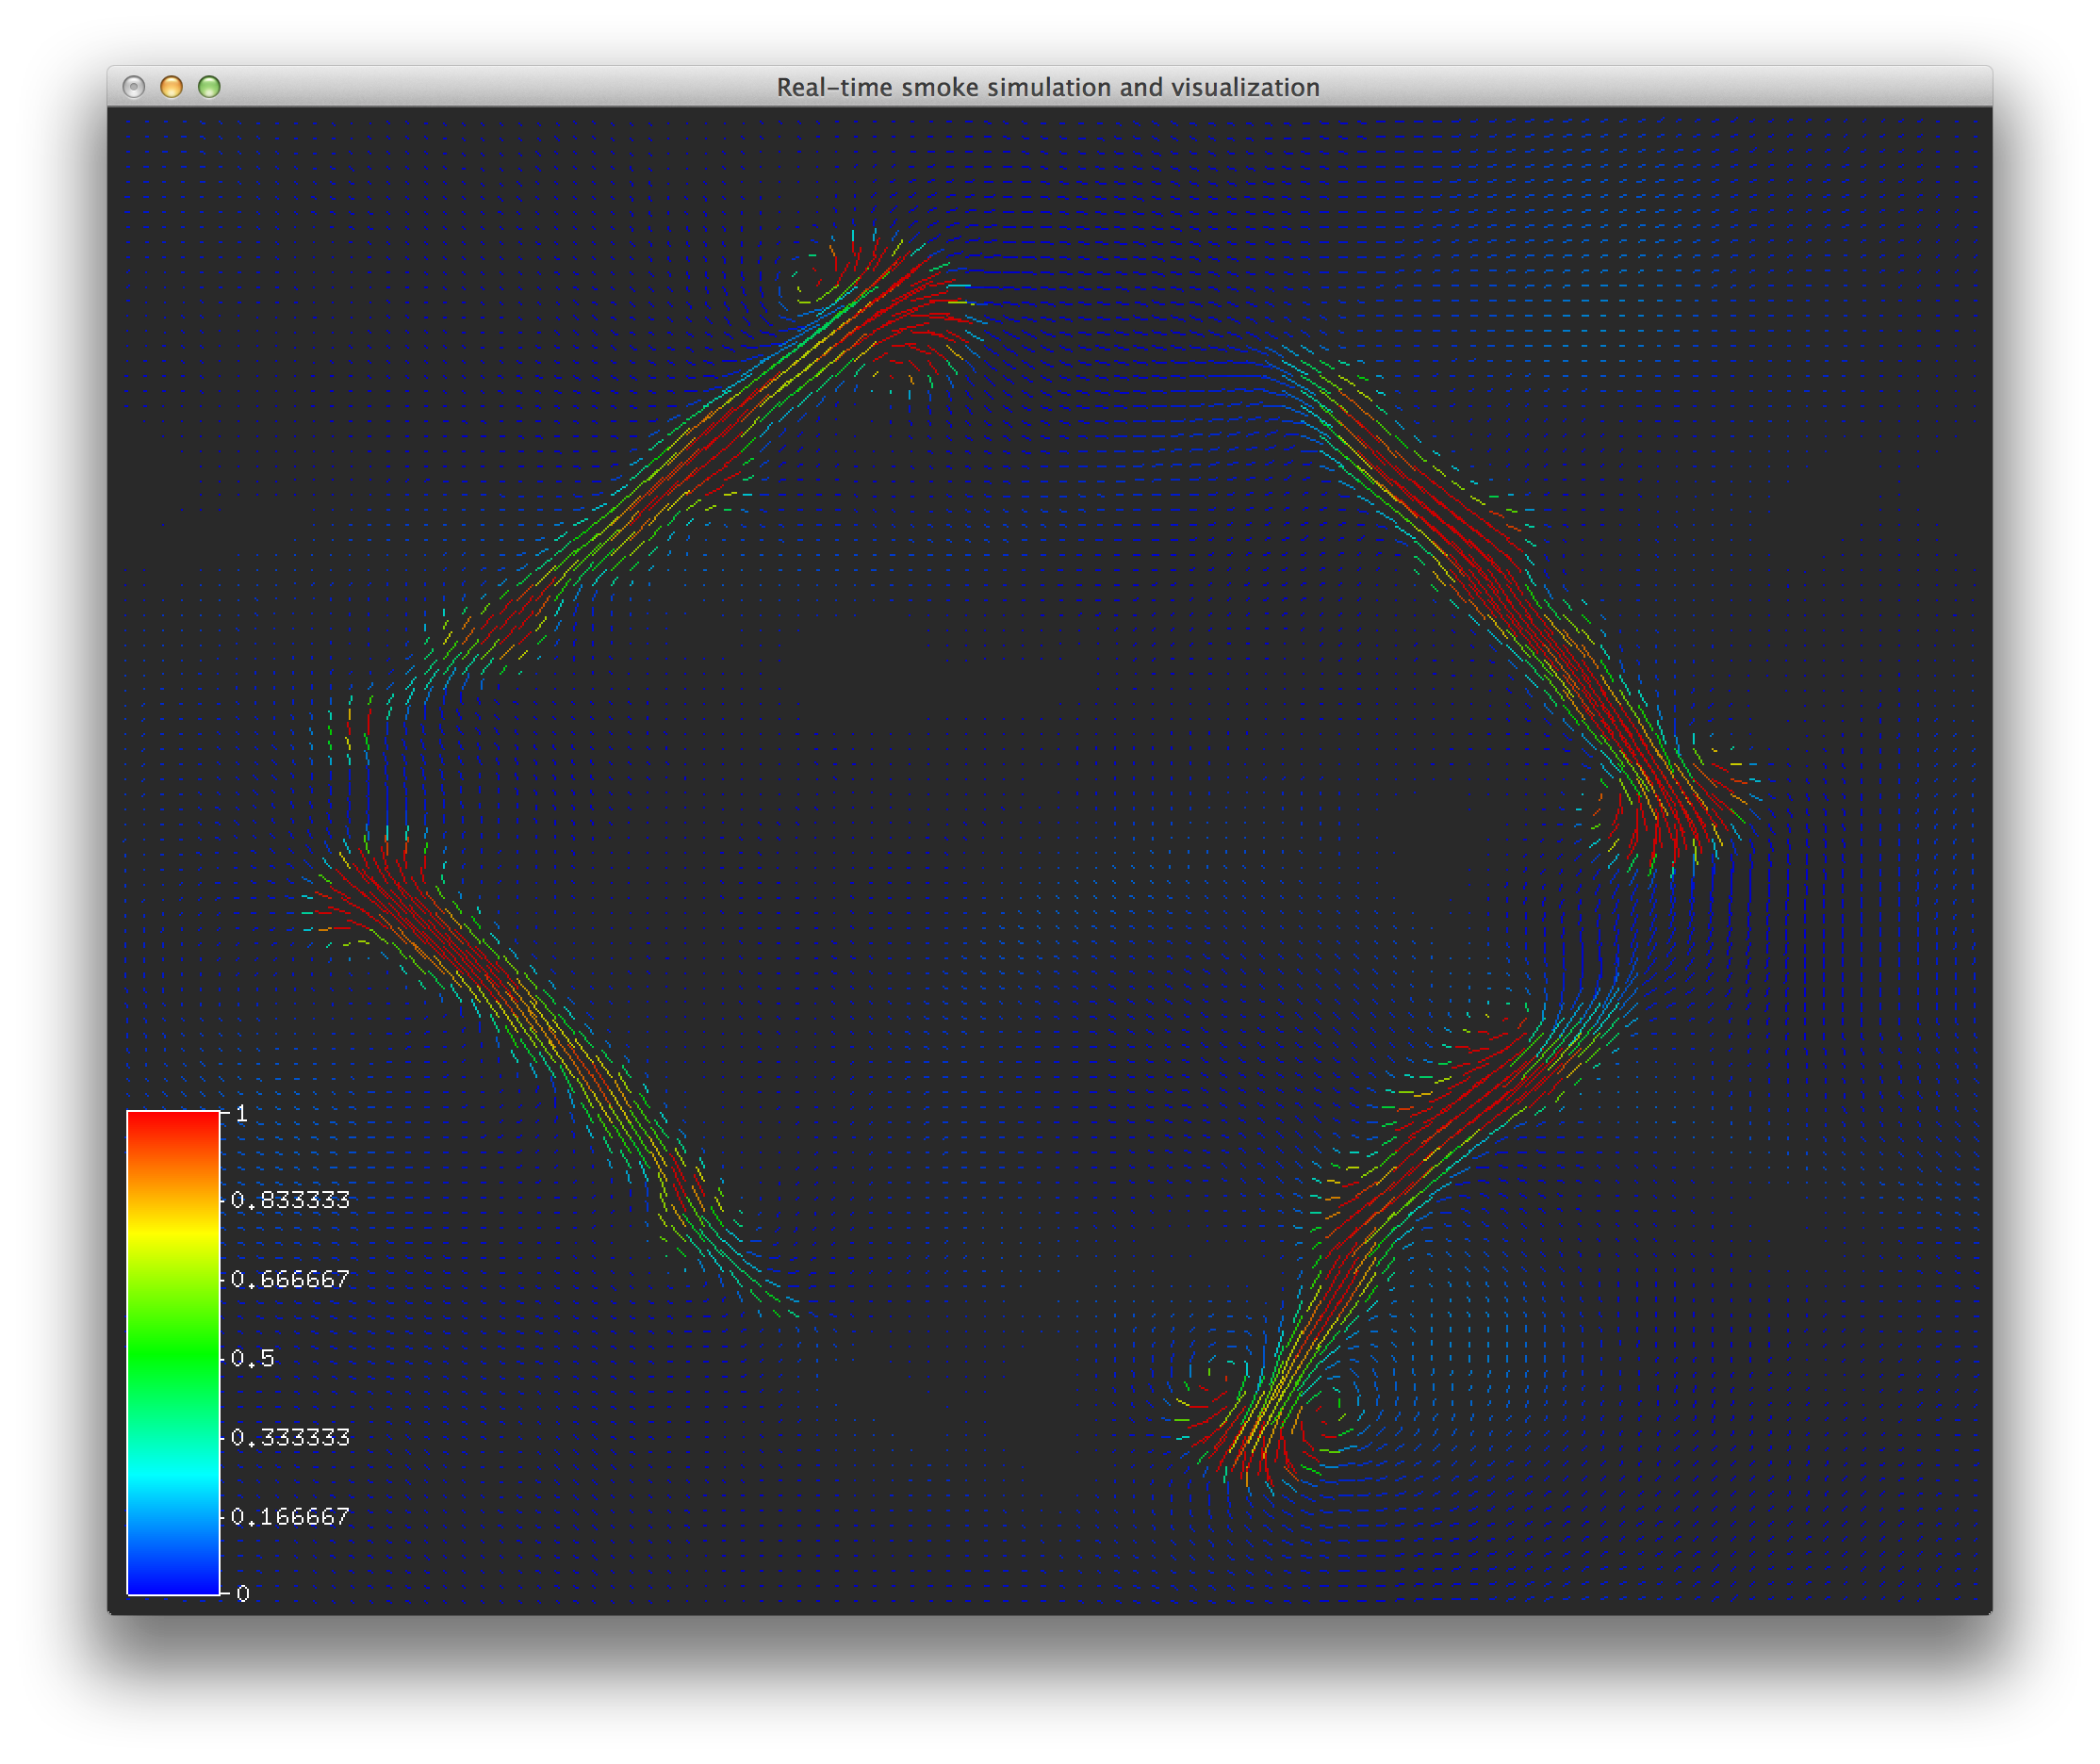
\includegraphics[height=2.7in]{figures/glyph/hedgehogsMSDSF.png}
\end{minipage}
\caption{Hedgehog visualisation of smoke simulation using rainbow colouring. (a) Regularly sampled on 40x40 and 200 scaling factor. (b) Regularly sampled on 100x100 and scaling factor 1000.}
\label{fig:hedgehogsSamplesScaling}
\end{figure}

Another possibility to avoid cluttering is to subsample the grid. For subsampling the grid, the user can select different values for the number of samples in the X dimension and the number of samples in the Y dimension. This can be done from the \emph{X Sample} and \emph{Y Sample} spinners respectively. When the grid is subsampled, the method of \emph{bilinear interpolation} is used in order to compute the dataset values out of the neighbour points.

Figure~\ref{fig:hedgehogsSubsampled} shows the same dataset as in Figure~\ref{fig:hedgehogsSamplesScaling}(b) this time subsampled to 40x40 samples per dimension from 100x100. It is clear that by subsampling the grid, the cluttering effect considerably decreases. Except from subsampling, there is also the option of supersampling. However, this technique would be used when the sampled dataset did not contain enough dataset points to draw our conclusions out of the visualisation. As this is not the case in our application we do not demonstrate it.

\begin{figure}[htbp]
\begin{center}
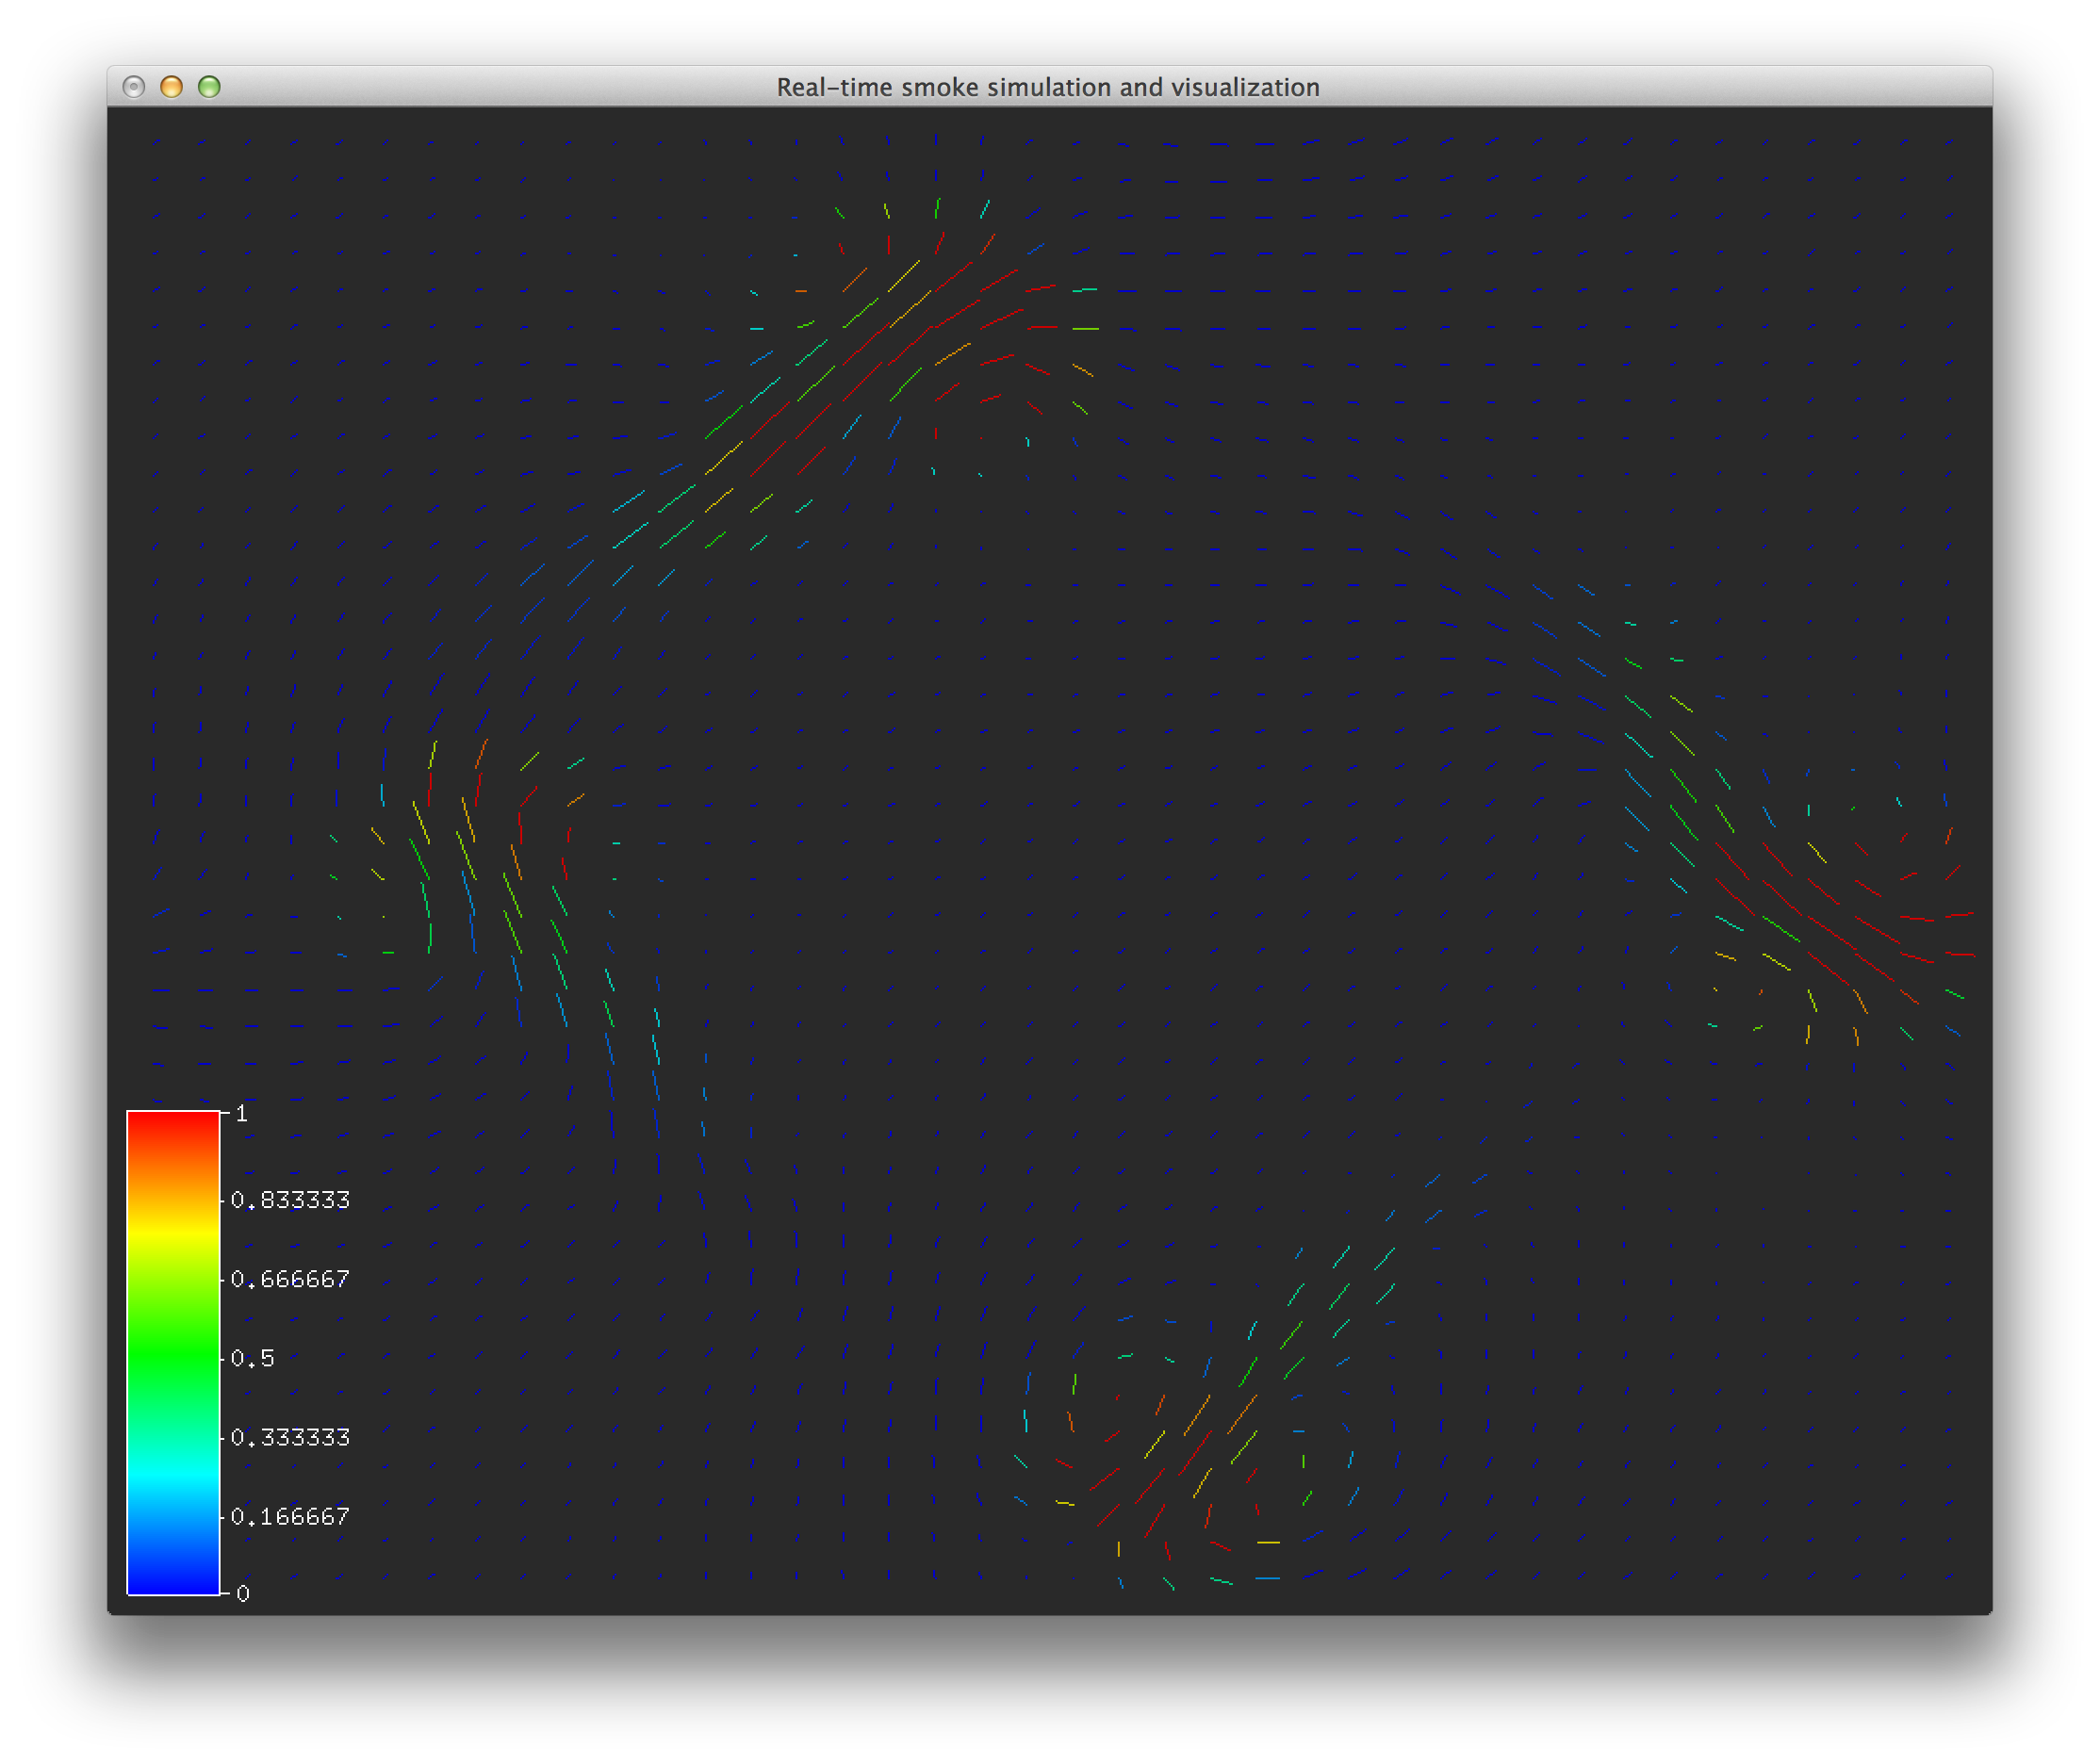
\includegraphics[height=3.5in]{figures/glyph/hedgehogsSubsampled.png}
\caption{Hedgehog visualisation of smoke simulation using rainbow colouring. Subsampled from 100x100 to 40x40.}
\label{fig:hedgehogsSubsampled}
\end{center}
\end{figure}

One disadvantage of hedgehogs is that they are not able to show orientation. The next three kinds of glyph icons have properties that are able to also convey the orientation of a vector dataset. However, when selecting glyph icons that need much more screen space than hedgehogs to be drawn, someone needs to think much more carefully about the design of these glyphs. Figure~\ref{fig:simpleArrowsCluttering}(a) depicts the sample dataset as in Figure~\ref{fig:hedgehogs}, this time with 2D arrows and texture color-mapping. Cluttering becomes much more apparent in case of using 2D arrows as glyphs, as it is also depicted in Figure~\ref{fig:simpleArrowsCluttering}(b). The scaling factor is 2 times larger and the length is scaled linearly with the vector magnitude.

\begin{figure}[htbp]
\centering
\begin{minipage}[t]{0.48\textwidth}
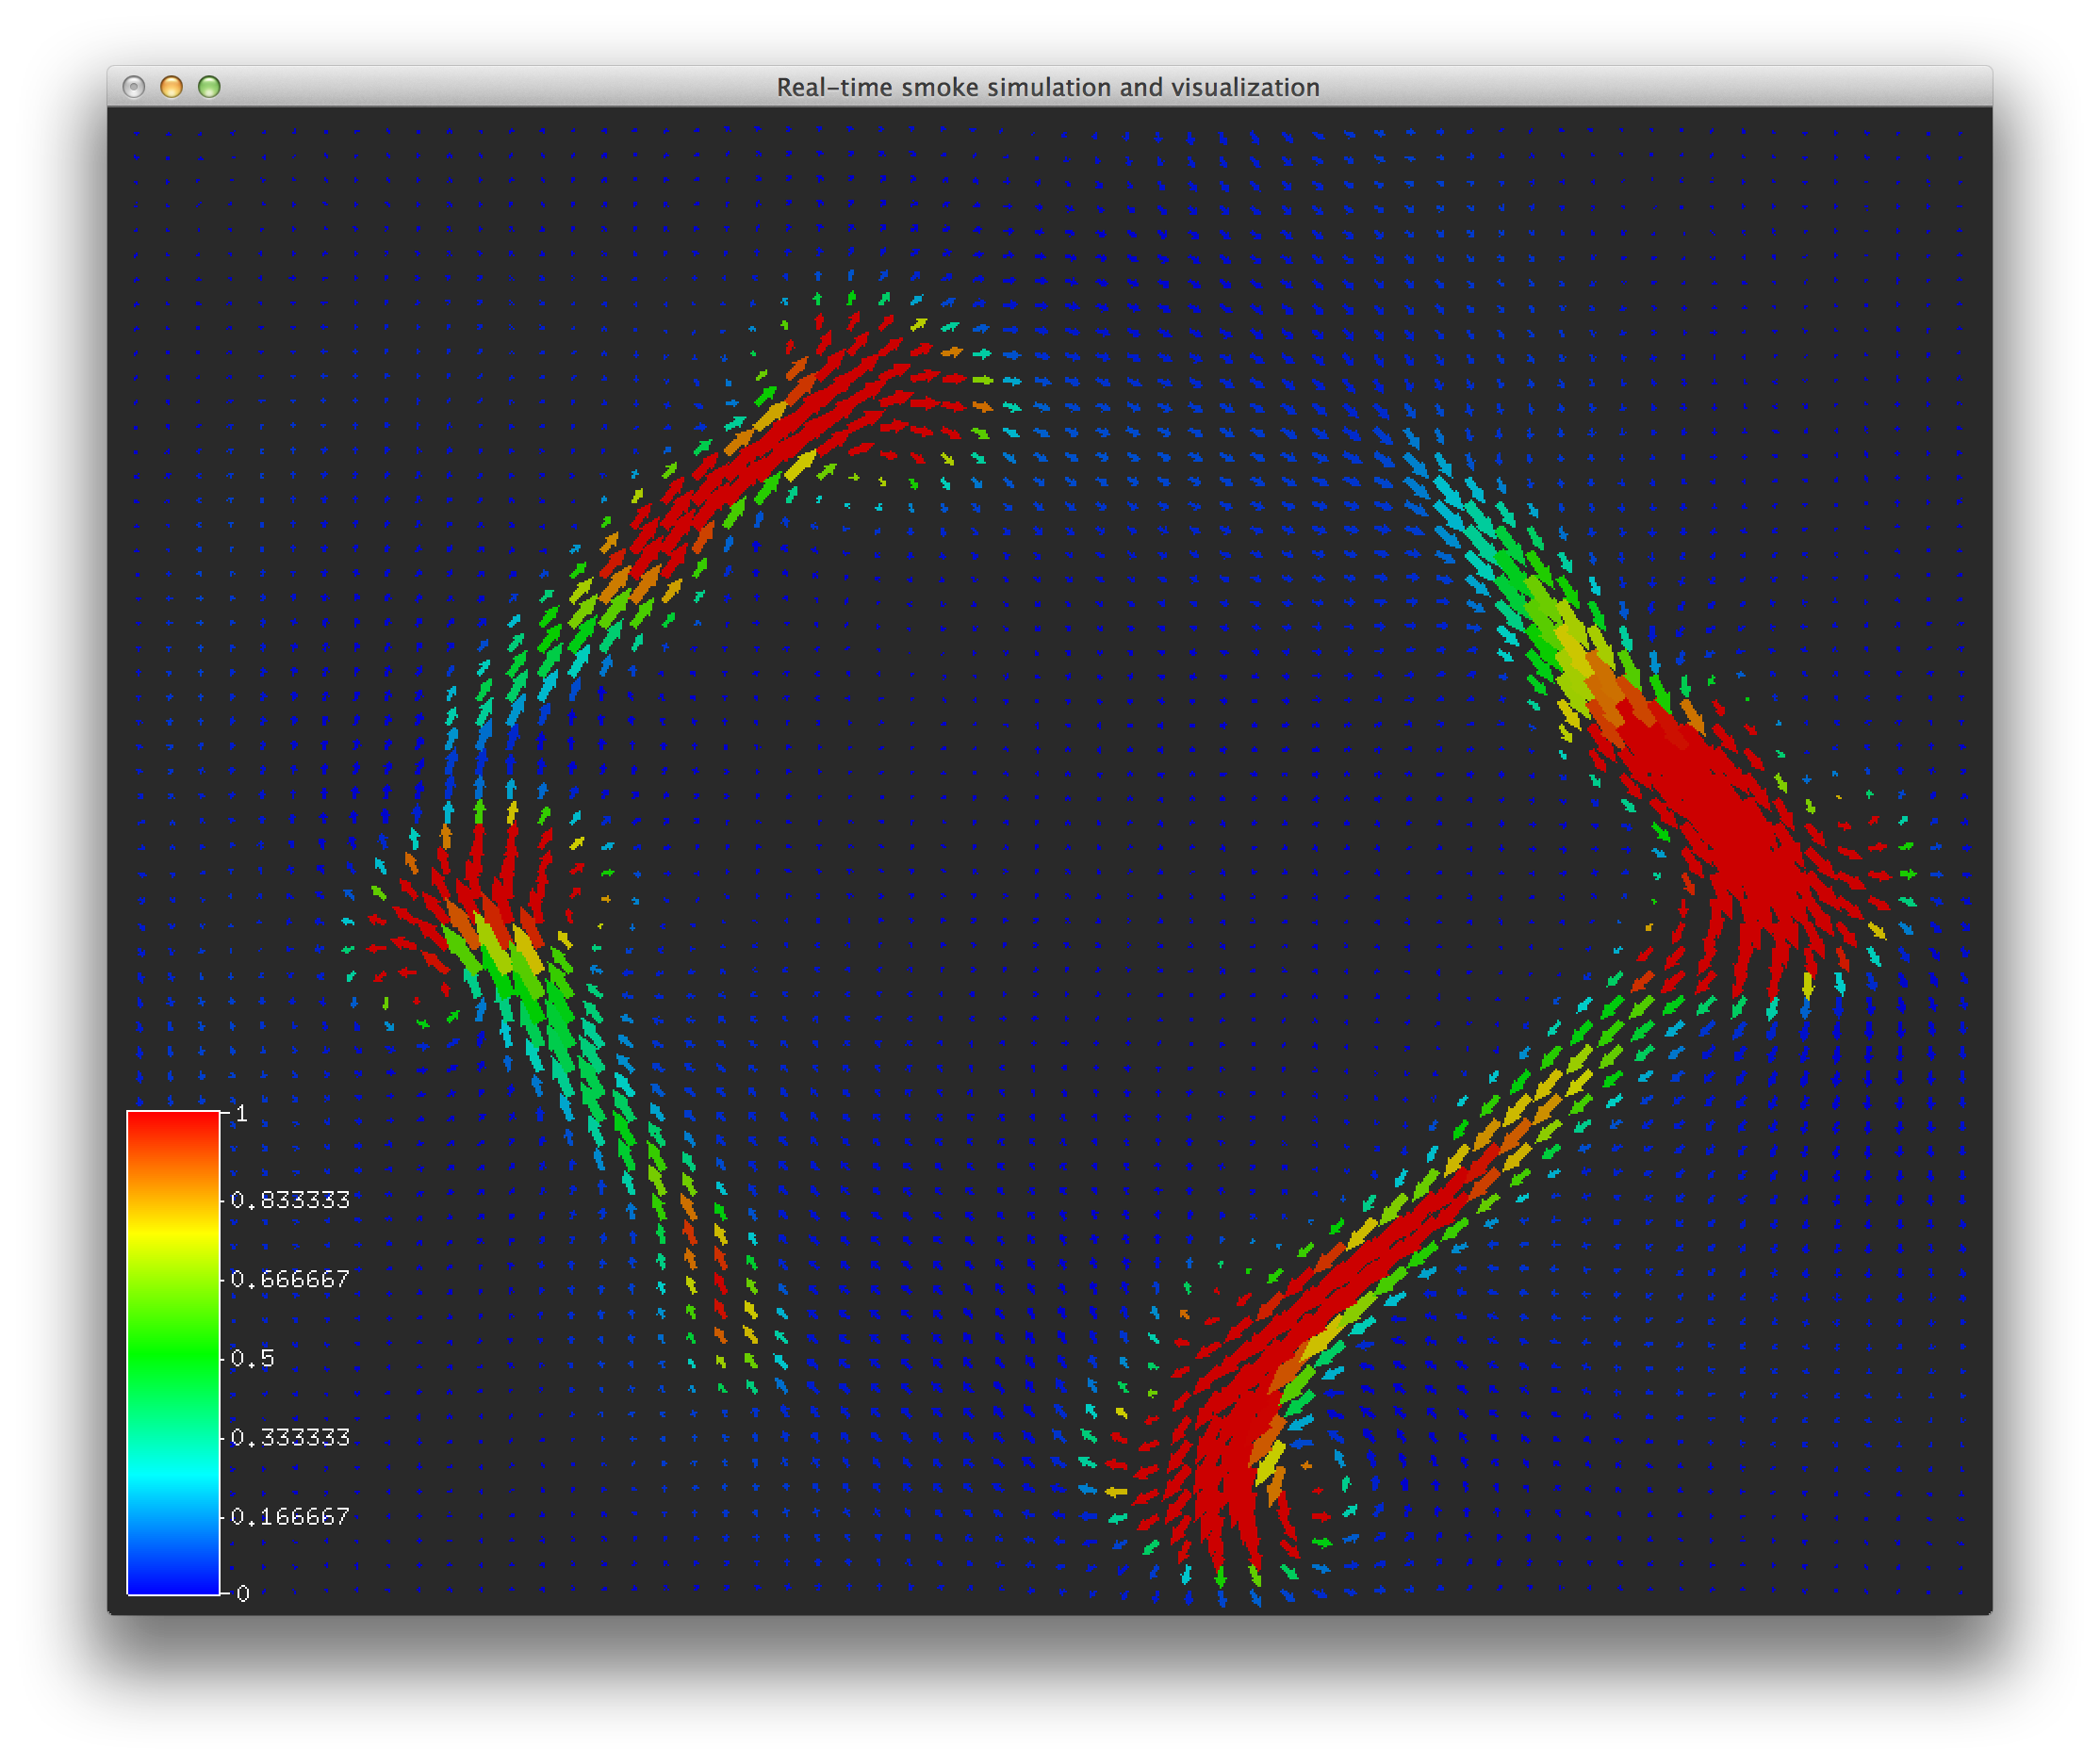
\includegraphics[height=2.7in]{figures/glyph/simpleArrows.png}
\end{minipage}
\begin{minipage}[t]{0.48\textwidth}
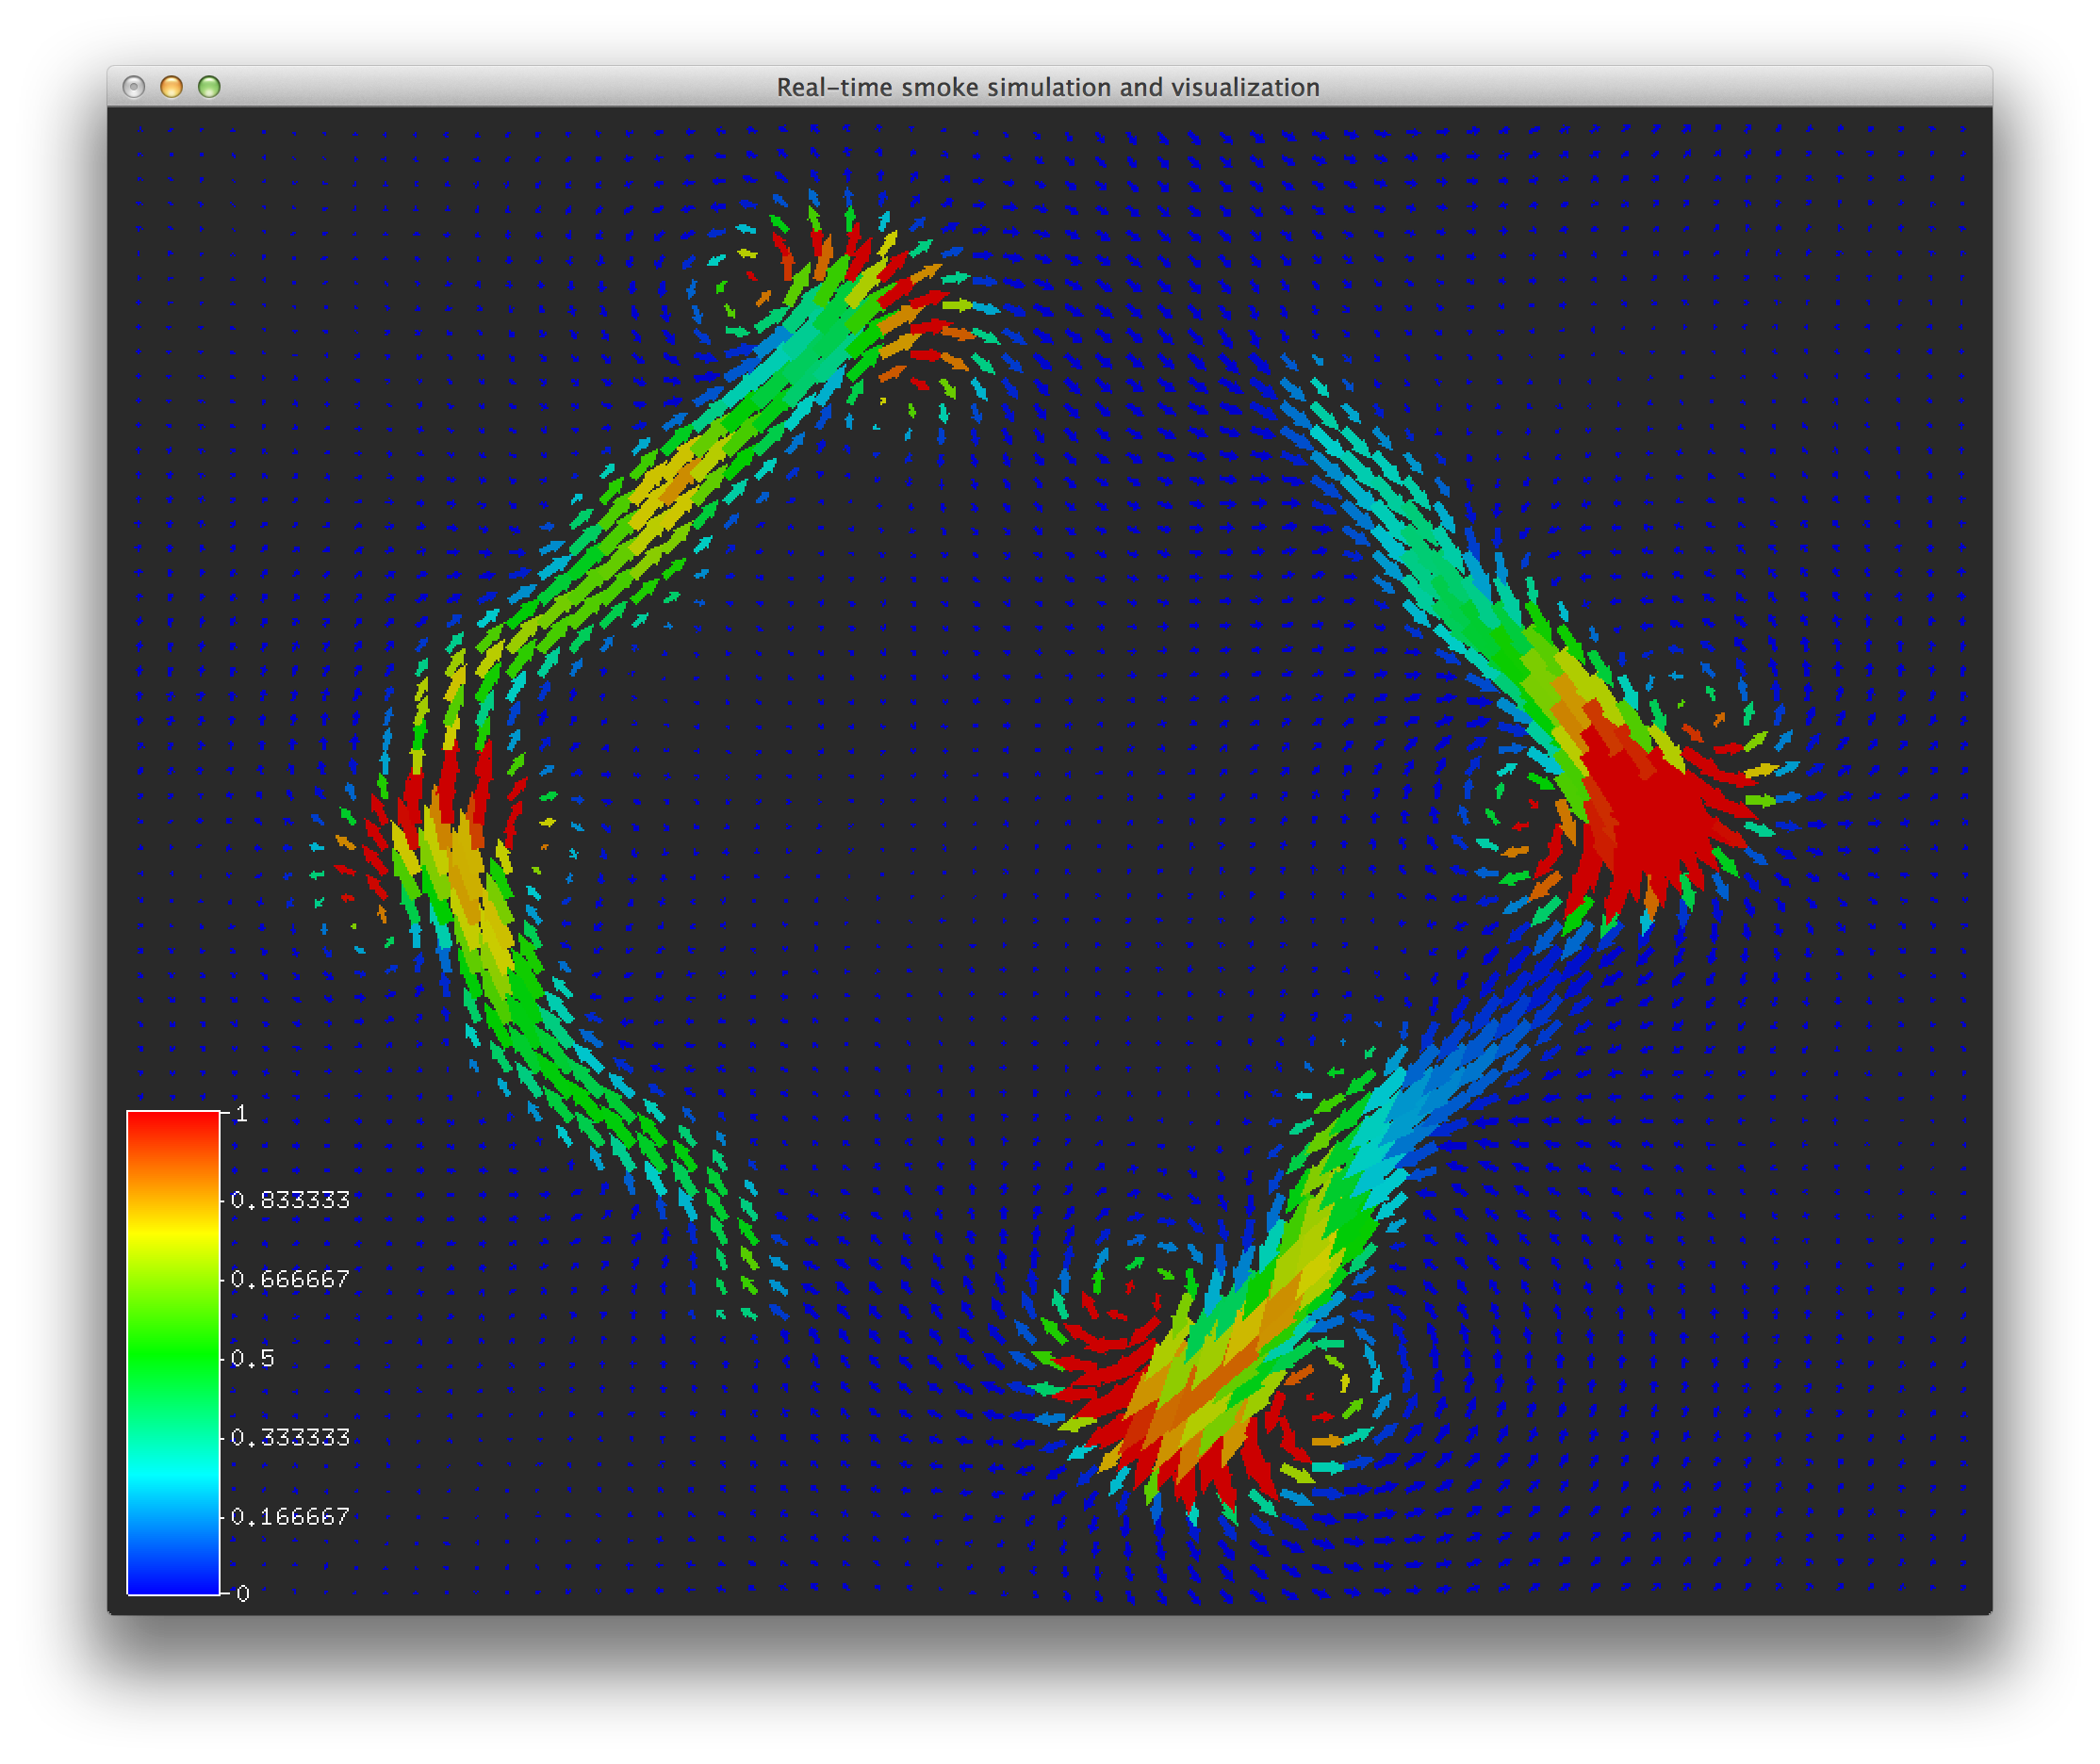
\includegraphics[height=2.7in]{figures/glyph/simpleArrowsScaled.png}
\end{minipage}
\caption{Simple arrows visualisation of smoke simulation using rainbow colouring. Regularly sampled to 60x60. (a) Normal scaling factor. (b) 2 times larger scaling factor.}
\label{fig:simpleArrowsCluttering}
\end{figure}

Another option would be to clamp the length of the arrows according to the size of the grid cells. The maximum values would be the maximum cell size and the minimum clamp values would be for instance 1/3 of the cell size. By trying out this technique we decided that in order to clamp the values to the grid cell size we would need to subsample the dataset so the cell size would increase and so the length of the arrows. In this way the length would indeed be a useful cue. However we decided that by visualising the field with more glyphs we can get a better insight into the visualised phenomenon. Figure~\ref{fig:d3conesArrows} illustrates the rest two kind of 3D glyphs visualising the dataset from Figure~\ref{fig:hedgehogs}. We should note that in order for the shading effect to work properly when visualising 3D glyphs, we set proper lighting source. The 3D glyphs exhibit the same issues as simple arrows upon visualisation, such as cluttering.

\begin{figure}[htbp]
\centering
\begin{minipage}[t]{0.48\textwidth}
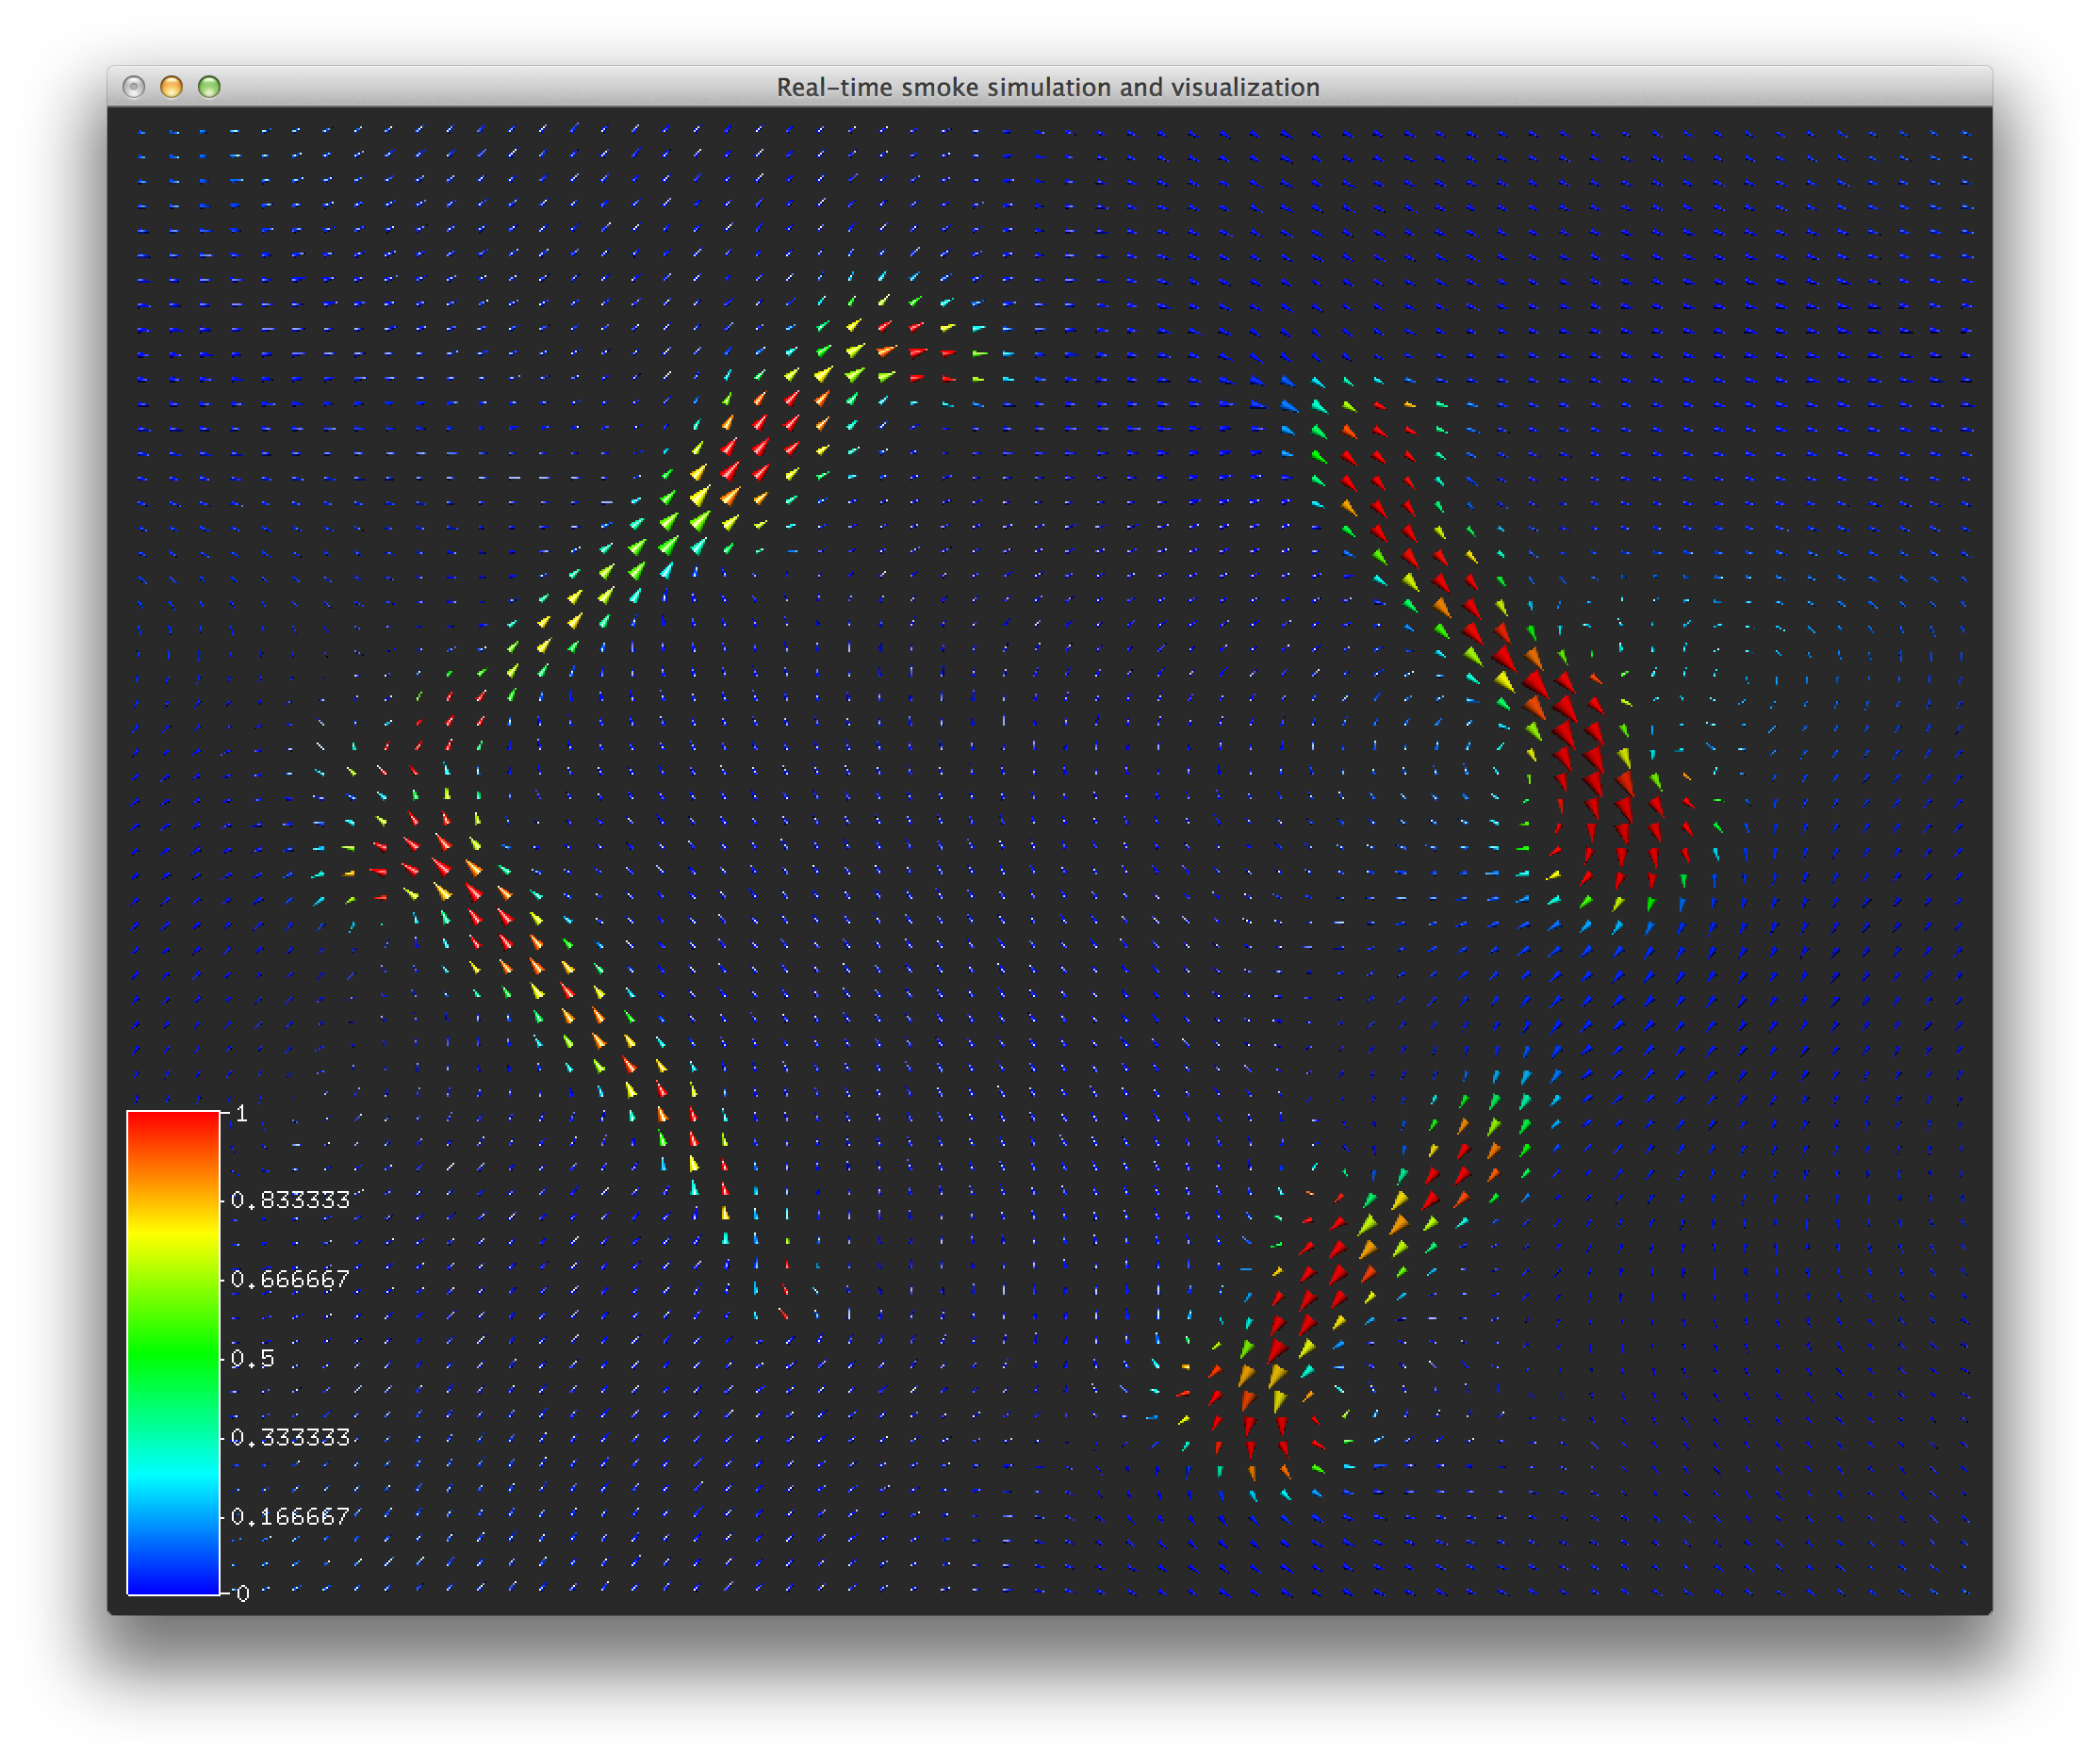
\includegraphics[height=2.7in]{figures/glyph/d3cones.png}
\end{minipage}
\begin{minipage}[t]{0.48\textwidth}
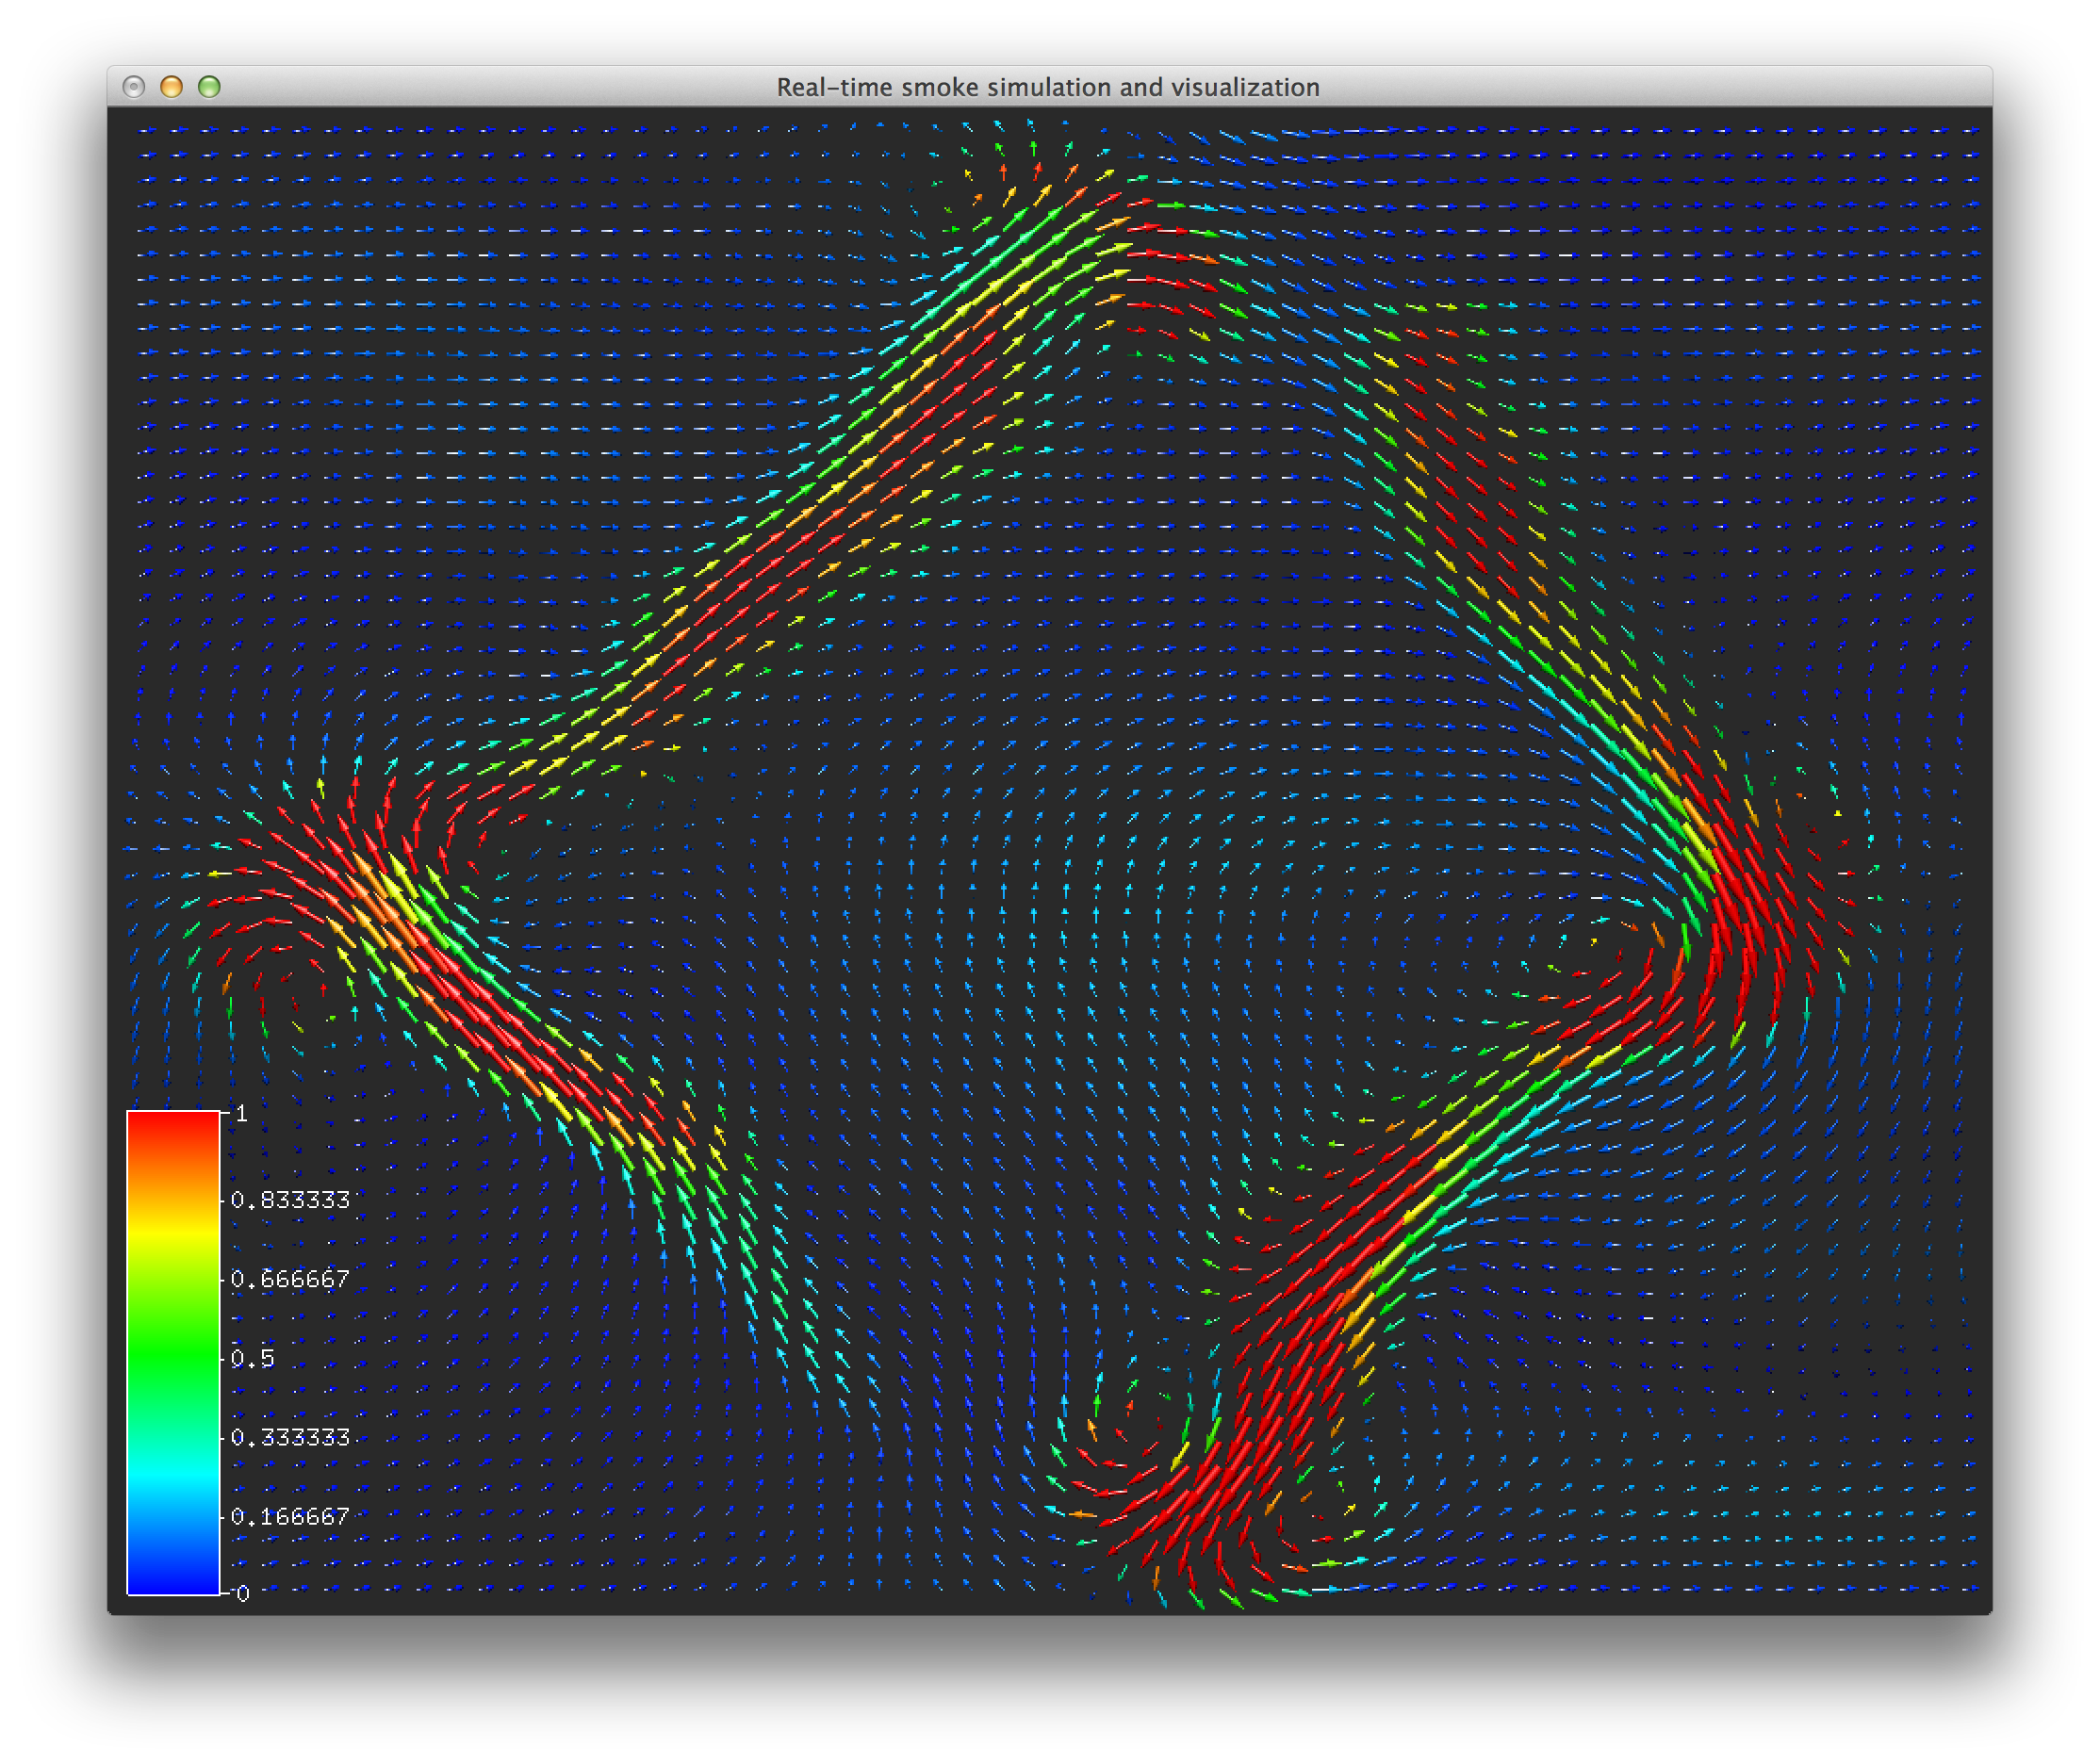
\includegraphics[height=2.7in]{figures/glyph/d3arrows.png}
\end{minipage}
\caption{3D Cones and Arrows visualisation of smoke simulation using rainbow colouring. Regularly sampled to 60x60.}
\label{fig:d3conesArrows}
\end{figure}

%The dataset class, separation of concerns, map that stores vector and scalar dataset, max and min for colormap
%changing the viewport to 3D

%vector interpolation (cf. exam question)

%design of glyphs, factor, orientation
%three-dimensional cones
%three-dimensional ellipsoids
%three-dimensional arrows consisting of a cone tip and a cylindrical shafts
%arrows implemented as two-dimensional nice-looking, high-quality, textures instead of simple polygonal shapes
%Consider carefully the glyph design: How thick to make the glyph? How long to make it? Should you scale the length linearly with the vector magnitude, or use another scale? Should you clamp the glyph’s minimal and maximal sizes to some values? If so, which are those?
%
%
%combining color mapping and glyphs
%difficulties with colorizing glut objects


%\begin{figure}[htbp]
%\centering
%\begin{minipage}[t]{0.48\textwidth}
% 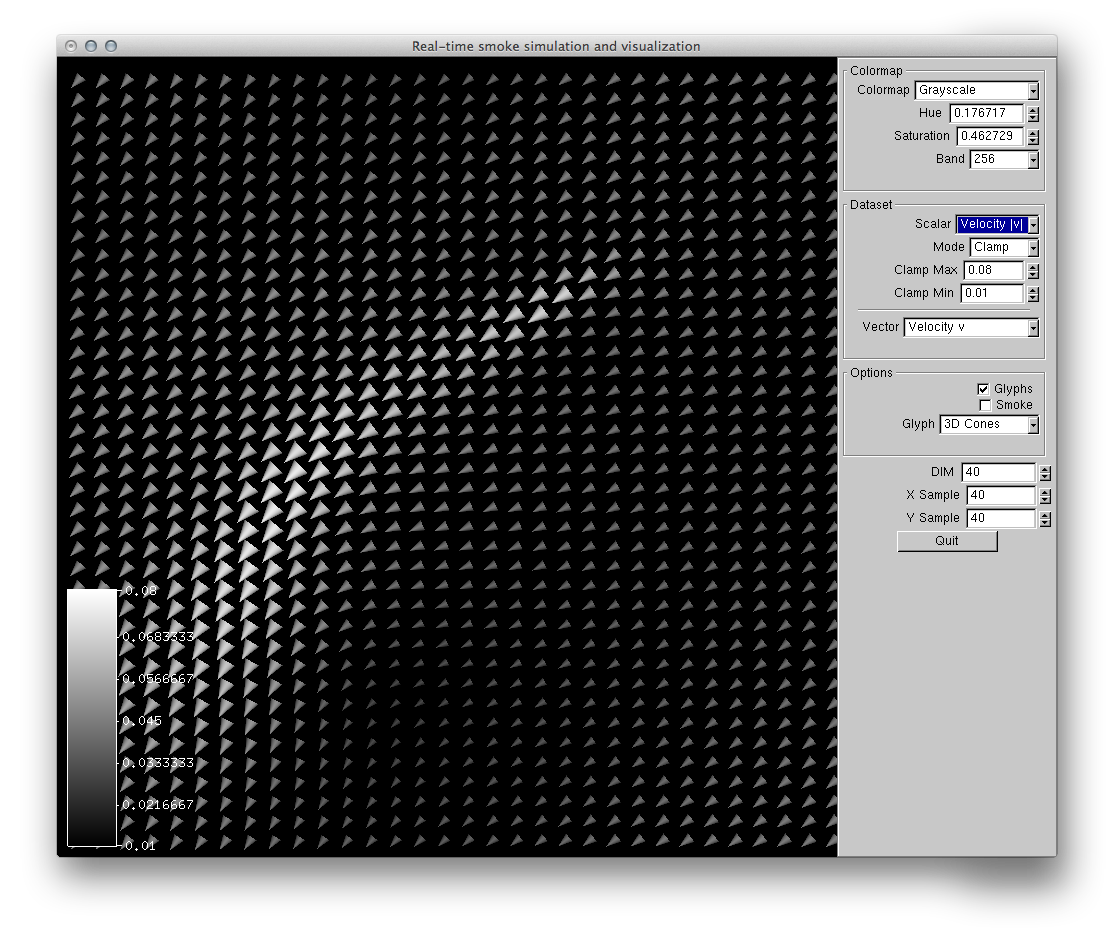
\includegraphics[height=3in]{figures/glyph/conesVelocityGrayscale.png}
%\caption{}
%\label{fig:forceScaled}
%\end{minipage}\hspace{.04\textwidth}%
%\begin{minipage}[t]{0.48\textwidth}
%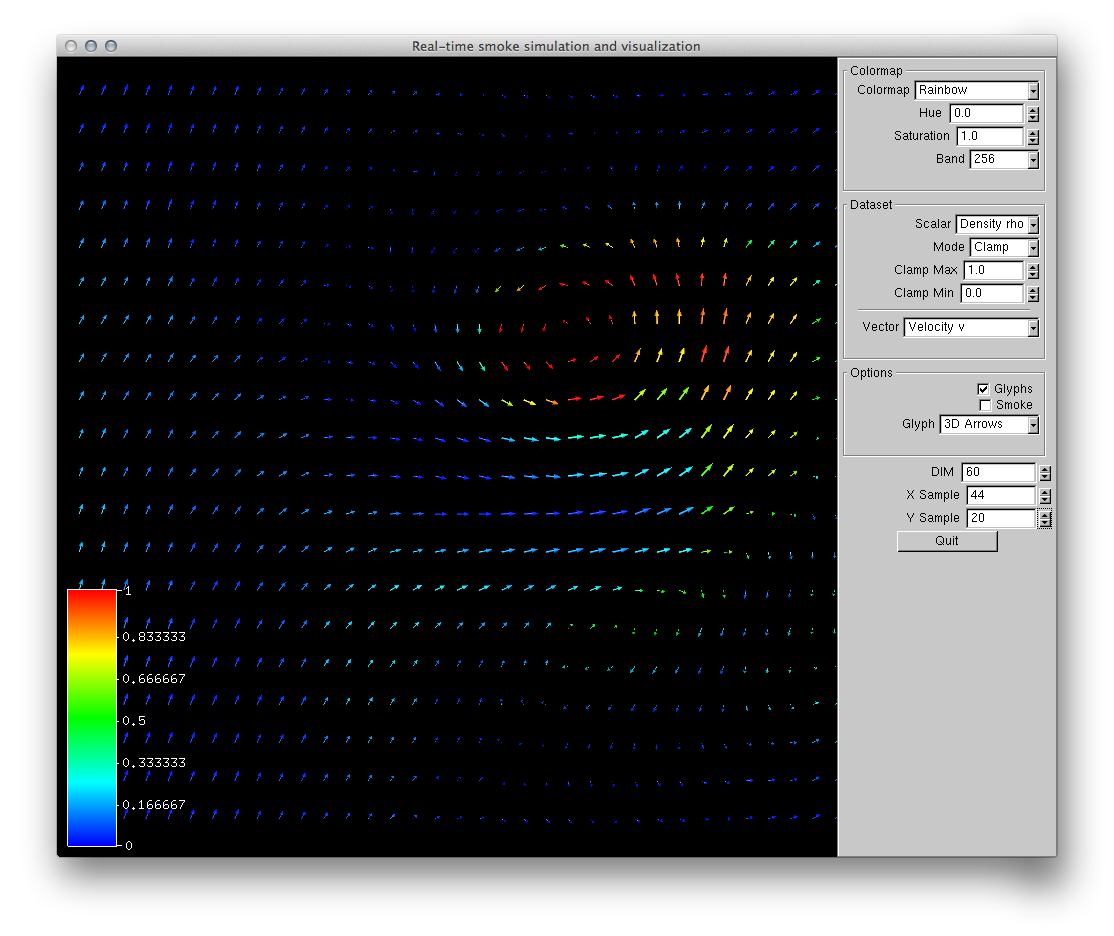
\includegraphics[height=3in]{figures/glyph/arrowsDensityVelocityRainbow.png}
%    \caption{}
%    \label{}
%\end{minipage}
%\end{figure}


